\documentclass{article}

\usepackage{graphicx} % Required for inserting images
\usepackage{amsfonts}
\usepackage{amsmath}
\usepackage{amssymb}
\usepackage{amsthm}
\usepackage{dirtytalk}
\usepackage{dsfont}
\usepackage{comment}
\usepackage{hyperref}
\usepackage{subcaption}
\usepackage{dirtytalk}
\usepackage{listings}
\usepackage{parskip}
\usepackage{bm}
\usepackage{bbm}
\usepackage[section]{placeins}
\usepackage[a4paper, margin = 1.3in]{geometry}
\renewcommand{\qedsymbol}{\ensuremath{\blacksquare}}

\usepackage{xcolor}

\definecolor{codegreen}{rgb}{0,0.6,0}
\definecolor{codegray}{rgb}{0.5,0.5,0.5}
\definecolor{codepurple}{rgb}{0.58,0,0.82}
\definecolor{backcolour}{rgb}{0.95,0.95,0.92}


\usepackage{fontspec}
\setmonofont{Iosevka NF}
%\setmonofont{IBM Plex Mono}

\lstdefinestyle{mystyle}{
	backgroundcolor=\color{backcolour},   
	commentstyle=\color{codegreen},
	keywordstyle=\color{magenta},
	numberstyle=\tiny\color{codegray},
	stringstyle=\color{codepurple},
	basicstyle=\ttfamily\footnotesize,
	breakatwhitespace=false,         
	breaklines=true,                 
	captionpos=b,                    
	keepspaces=true,                 
	numbers=left,                    
	numbersep=5pt,                  
	showspaces=false,                
	showstringspaces=false,
	showtabs=false,                  
	tabsize=2,
    % lineskip={-1pt},
    % columns=fullflexible
}

\lstset{style=mystyle}



\newtheorem{theorem}{Theorem}
\newtheorem{definition}{Definition}
\newtheorem{proposition}{Proposition}
\newtheorem{lemma}{Lemma}
\newtheorem{example}{Example}
\newtheorem{corollary}{Corollary}
\newtheorem{remark}{Remark}
\usepackage[backend=biber,style=numeric]{biblatex}
\addbibresource{references.bib}

\DeclareMathOperator{\Cov}{Cov}
\DeclareMathOperator{\Corr}{Corr}
\DeclareMathOperator{\Var}{Var}

\setlength{\parindent}{0pt}
\setlength{\parskip}{8pt}

\title{Quantitative Risk Measurement}
\author{Simeon Duwel, Mara Levrau}
\date{March 2026}

\begin{document}

\maketitle

\section*{Inleiding}
Kwantitatieve risicoanalyse is een parapluterm voor een verscheidenheid aan technieken die gebruikt worden om potentiële verliezen te kwantificieren, voornamelijk in een actuariële of financiële context. Men kan zich een verzekeraar of bank inbeelden, die polissen afsluit of leningen aangaat, met daaraan geassocieerd een bepaald `risico' om een verlies te moeten incasseren: dit komt voor als de polishouder een schadeclaim indient, of als de lener de lening niet terug kan betalen. In het algemeen is een verzekeraar niet zozeer geïnteresseerd in individuele risico's, maar eerder in hun aggregaat, i.e. de som van alle individuele risico's voor alle polishouders. Het is immers precies dit totale risico dat bepaalt hoeveel reservekapitaal de verzekeraar moet bezitten, teneinde de verwachte claims terug te kunnen betalen (dit bedrag heet ook wel het \textit{technische reservekapitaal}).

Als we $n$ klanten hebben, ieder met een geassocieerde stochastische variabele $X_i$ (waarbij \mbox{$i \in \{1, ..., n\}$}) die het risico van die klant beduidt, noteren we het geaggregeerde risico met \mbox{$S = \sum_{i=1}^n X_i$}. Als we eigenschappen over $S$ willen afleiden, is het wiskundig gesproken het eenvoudigst als alle $X_i$'s onafhankelijk zijn. In de praktijk is dit zelden tot nooit het geval: als er bijvoorbeeld in een wijk een huisinbraak voorkomt, kan dit een goede indicatie zijn dat nabijgelegen huizen in die wijk in de nabije toekomst ook bestolen zullen worden. We willen die afhankelijkheidsstructuur tussen de verschillende risico's dus modelleren op een wiskundig haalbare manier. Teneinde zo'n modellering te bewerkstelligen, introduceren we een bepaalde klasse verdelingsfuncties, \textit{copulae} geheten.

In dit document zal onze focus liggen bij het specifieke geval waarbij de indiviuele risico's lognormaal verdeeld zijn (dat wil zeggen: de logaritmes van de risico's in kwestie zijn normaal verdeeld), en de copula tussen deze verliezen de zogeheten Gaussische copula is. Ons doel zal eruit bestaan een adequate benadering voor $S$ te vinden, als een gesloten uitdrukking. We zullen de rekentijden en accuraatheid van deze gesloten vorm dan vergelijken met die van de `primitievere' Monte Carlomethode.

\subsection*{Algemene context}
Doorheen dit verslag zullen we ons het perspectief van een verzekeringsmaatschappij. Het is natuurlijk de primaire interesse van dit bedrijf om winst te maken. In een ietwat vereenvoudigde visie kan dit enkel gebeuren als het kan garanderen dat de geldsom die door polishouders geclaimd wordt, de totale inkomsten niet overstijgt. Die totale inkomsten worden op hun beurt bepaald door de prijs van de polissen die het bedrijf afsluit (dit bedrag heet de \textit{verzekeringspremie}). Het kerndoel is dus om te bepalen hoeveel geld we ``opzij moeten houden'', om te claims te kunnen betalen die we verwachten binnen te krijgen. Veronderstel dat we $n$ polishouders hebben. Elk van die polishouders kan aan de hand van een stochastische variabele $X_i$ gemodelleerd worden, waarbij de waarde van die variabele voorstelt hoeveel geld deze polishouder claimt. Elk van deze variabelen noemen we een \textit{risico}. Wij zijn geïnteresseerd in het \textit{geaggregeerde risico}, aangeduid met $S$ en gedefinieerd als $\sum_{i=1}^n X_i$, en in het bijzonder in de verwachtingswaarde $\mathbb{E}[S]$. Immers, als de verzekeringsmaatschappij zich ervan vergewist steeds over deze geldsom te beschikken, verwachten we dat alle gemaakte claims uitbetaald kunnen worden. Dit totale risico heet het \textit{technische reservekapitaal}. 

Onder de aanname dat alle claims onafhankelijk zijn (in de kansrekeningszin van het woord), is de berekening van deze verwachtingswaarde in de praktijk zeer eenvoudig, aangezien we eenvoudigweg de som van de individuele verwachtingswaarden kunnen nemen. Maar in de praktijk kunnen we zo'n aanname niet maken: bijvoorbeeld natuurrampen kunnen schade aanrichten in een groot gebied, waardoor er veel claims over huisvestingsschade tegelijkertijd binnen zullen komen.

We zullen in dit verslag ook enkele risicomaten bespreken. In actuariële context is dit vooral relevant omdat financiële controleorganen bepaalde vereisten opleggen aan verzekeringsmaatschappijen omtrent een minimumkapitaal dat ze verplicht zijn te bezitten. Dit minimumkapitaal wordt berekend aan de hand van die zogeheten risicomaten. Er is echter een kost verbonden aan meer kapitaal verwerven (omwille van investeringsgerelateerde kwesties), dus is het voor een verzekeraar vaak een delicate balans. In het bijzonder wordt de zogeheten \textit{Value-at-Risk} gebruikt in wetgeving.

\subsection*{Verwachtenutstheorie}
Het klassieke raamwerk voor redeneringen over de rationaliteit van beslissingstheorie werd omstreeks de jaren '50 door John von Neumann en Oskar Morgenstern geopperd. Centraal in hun redenering is het concept van een \textit{nutsfunctie} $u: \mathbb{R} \to \mathbb{R}$ die de mate vat waarin de agent in kwestie het vergaren van een bepaalde hoeveelheid kapitaal waardeert, hoeveel `nut' die hoeveelheid kapitaal heeft. Von Neumann en Morgenstern poneren dat elke ``rationele'' agent een intrinsieke nutsfunctie heeft, die gebruikt wordt om een redelijk actieplan op te stellen: de rationele keuze is precies die keuze wiens uitkomst de verwachtingswaarde van de nutsfunctie maximaliseert.  Als een nutsfunctie concaaf is (i.e. gedefinieerd op een compactum $I$ van $\mathbb{R}$ zodat $\forall x, y \in I, \forall t \in [0, 1]: u(tx + (1-t)y) \geq t u(x) + (1-t) u(y)$), noemen we de agent \textit{risico-avers}.

\newpage

\section{Introduction}
Quantitative risk measurement is an umbrella term for a variety of techniques used to quantify potential losses, often in an actuarial or financial context. One can imagine an insurer or a bank writing out premiums or loans, with a certain associated `risk' of incurring a loss: either the policyholder files a claim, or the lender cannot pay back their loan. An insurer is in general not interested in individual risks, but in their aggregate: indeed, it is the total risk that determines the necessary reserves the insurer needs to put aside, to pay out the claims that they expect to receive (the so-called \textit{technical reserves}).

If we have $n$ clients, each with an associated random variable $X_i$ (for $i \in \{1, ..., n\}$) representing the risk of this client, the aggregate risk is denoted with $S = \sum_{i=1}^n X_i$. The mathematics for working out properties of $S$ is by far the easiest if all $X_i$'s are independent, but this is in practice rarely the case: for example, a burglary occurring in a neighbourhood can be a good indicator of other houses in the same neighbourhood being burgled in a short timespan after the first incident. As a result, we want to model the dependence structure between the different risks, in a way that is mathematically still feasible. To this end, we introduce a special class of distribution functions called \textit{copulas}.

In this document, our focus will be on the specific case where our losses are distributed lognormally, and the copula between these losses is the so-called Gaussian copula. Our goal will be to find an adequate approximation for $S$, in a closed form expression. We will numerically compare the calculation speeds and accuracy of this closed form with the more ``primitive'' Monte Carlo method.

\subsection{General context}
Throughout this report, we will be placing ourselves in the shoes of an insurance company. It is of course in the interest of this company to make a profit. In a simplified view, it can only do so if it can make sure that the sum of money that is claimed by the policyholders does not exceed the total income, which in turn is determined by the price of the insurance policies that the company decides to offer (this price is called the policy's \textit{premium}). The core objective is thus to determine how much money to put aside, to pay out the claims the company expects to receive. Suppose we have $n$ policyholders. Each of the policyholders can be modelled using a stochastic variable $X_i$ (with $1 \leq i \leq n$), where the value of this variable represents the amount of money that this client files a valid claim for. Each of these variables is called a \textit{risk}. We are interested in the \textit{aggregate risk}, denoted $S$ and defined as $\sum_{i=1}^n X_i$, and in particular the expected value $\mathbb{E}[S]$. Indeed, if the insurance company makes sure to have at least this sum of money, we can expect to cover the claims that will be made. This total risk is called a \textit{technical reserve}.

Under the assumption that all claims are independent of each other (in the probability theoretical sense), the calculation of this expected value is very easy in practice, since we can simply sum together the individual expectations. However, in practice one cannot make this assumption: for instance, natural disasters can wreak havoc in a large residential area, resulting in several claims relating to housing damage all at once.

In this report we will also discuss some risk measures. This is predominantly relevant in an actuarial context since financial regulators impose certain restrictions on insurers concerning a minimum capital that they are legally required to own. This minimum capital is often calculated based on these risk measures. However, there is a cost to accruing more capital (due to investment-related matters), so for insurers this is often a delicate balance. In particular the so-called \textit{Value-at-Risk} is often used in legislation.

\subsection{Expected utility theory} 
The classical framework used to reason about the rationality of making decisions was first proposed by John von Neumann and Oskar Morgenstern. Central in their reasoning is the concept of a \textit{utility function} $u: \mathbb{R} \to \mathbb{R}$, which quantifies the degree to which the agent under consideration values accruing a given amount of capital. Von Neumann and Morgenstern posit that any ``rational'' agent has an intrinsic utility function which they use to determine a reasonable course of action: the rational choice is precisely the choice whose outcome is expected to maximise the value of the agent's utility function. If a utility function is concave (i.e. defined on a compact set $I$ of $\mathbb{R}$ such that $\forall x, y \in I, \forall t \in [0, 1]: u(tx + (1-t)y) \geq t u(x) + (1-t) u(y)$), the corresponding agent is called \textit{risk averse}.



\section{Assumptions}\label{section: assumptions}
In this report we will assume that all random variables are defined on a common probability space $(\mathbb{R}, \mathcal{B}(\mathbb{R}),P)$. Additionally we suppose that the expectation $\mathbb{E}[X]$ exists and is finite for every random variable.

We will focus on the case where all the risks follow a lognormal distribution. In particular this means that the random variables that interest us have continuous cumulative distribution functions. Throughout this report we will only prove the relevant results for continuous random variables. In addition we will assume that all cumulative distribution functions $F$ have an interval $I = (a,b)\subseteq \mathbb{R}$ (where $a$ and $b$ are possibly infinite) such that the following holds:

\begin{itemize}
    \item $F$ is strictly increasing on $I$;
    \item $\lim_{x\rightarrow a^+} F(x) = 0$;
    \item $\lim_{x\rightarrow b^-} F(x) = 1$.
\end{itemize}

This implies that $F:I\rightarrow F(I)$ is a bijection and hence invertible. As a result of this assumption, we can define $F^{-1}(0) := a$ and $F^{-1}(1) := b$ (where $a$ and $b$ are possibly infinite) for every random variable with cumulative distribution function $F$.

It is important to note that most of these results still hold for discrete random variables. Most of these generalisations can be found in \cite{Risk_Measurement} and \cite{kaas-2000}, but this falls outside the scope of this report.

\section{Risk measures}

Risk measures are functions used for quantifying the risk inherent to a certain stochastic variable. One practical purpose of such quantification worth immediately highlighting here is to determine the minimum capital an insurance company is legally required to possess. For example, in the European Union, the Solvency II directive states that the ``solvency capital requirement [...] shall correspond to the Value-at-Risk of the basic own funds of an insurance or reinsurance undertaking subject to a confidence level of 99,5 \% over a one-year period'' \cite[Art. 101ter.]{SolvencyII}. This \textit{Value-at-Risk} is an example of a risk measure, which we define below.
\\
\begin{definition}\cite[Definition 6.2.1]{Risk_Measurement}
A risk measure $\rho$ is a real functional on a set of real-valued random variables $\Gamma$ on some probability space $(\Omega, \mathcal{F}, \mathbb{P})$. 
\end{definition}
This definition alone is much too general to derive useful results from; in practice we restrict $\Gamma$ to be (1) closed under addition, (2) closed under positive scalar multiplication and (3) translation-invariant. That is, $\forall X_1, X_2 \in \Gamma, a \in \mathbb{R}_{> 0}, b \in \mathbb{R}$, 
\begin{enumerate}
    \item $X_1 + X_2 \in \Gamma$,
    \item $a X_1 \in \Gamma$,
    \item $X_1 + b \in \Gamma$.
\end{enumerate}

A particular class of risk measures are the \textit{convex} risk measures. These are precisely those risk measures $\rho$ that are monotone (that is, $\forall \omega \in \Omega: X(\omega) \leq Y(\omega) \implies \rho[X] \leq \rho[Y]$), translation invariant ($\forall a \in \mathbb{R}, X \in \Gamma: \rho[X + a] = \rho[X] + a$) and convex ($\forall X, Y \in \Gamma, \lambda \in [0, 1]: \rho[\lambda X + (1-\lambda) Y] \leq \lambda \rho[X] + (1-\lambda)\rho[Y]$). A historically used set of extra requirements is that of positive homogeneity and subadditivity. A risk measure satisfying these requirements is called a \textit{coherent} risk measure. However, especially this latter requirement has been argued to be too strong a claim to make for reasonable use in financial mathematics, among others by Föllmer and Schied \cite{Follmer2002}. 

Let us now look at some examples of risk measures that we will encounter later.
\\
\begin{definition}\cite[Definition 6.3.1]{Risk_Measurement}
    For a given random variable $X$, the \textit{Value-at-Risk} at probability level $p \in (0, 1)$ is defined as $$\text{VaR}_p[X] := \inf \left\{x \in \mathbb{R} \mid F_X(x) \geq p \right\} = F_X^{-1} (p).$$
\end{definition}

\begin{definition}\cite[Definition 6.3.2]{Risk_Measurement}
    For a given random variable $X$, the \textit{Tail Value-at-Risk} at probability level $p \in (0, 1)$ is defined as $$\text{TVaR}_p[X] := \frac{1}{1 - p} \int_p^1  F_X^{-1} (q) \, \textrm{d}q.$$
\end{definition}

\begin{definition}\cite[Definition 6.3.4]{Risk_Measurement}
    For a given random variable $X$, the \textit{Expected Shortfall} at probability level $p \in (0, 1)$ is defined as $$\text{ES}_p[X] := \mathbb{E} \! \left[(X - F_X^{-1}(p))_+\right].$$
\end{definition}

One can prove that the Expected Shortfall and the Tail Value-at-Risk are related as follows:
$$\text{TVaR}_p[X] = F_X^{-1}(p) + \frac{1}{1-p}\text{ES}_p[X]$$
for $p\in (0,1)$.

Intuitively, one can think of the Value-at-Risk as the quantity that answers the question ``What loss is exceeded with probability $1 - p$?'', whereas the Tail Value-at-Risk answers the question ``How bad is the situation once we indeed exceed that $1-p$ loss?'' This highlights one of the most often criticised weaknesses of the VaR: in a sense, it is not sensitive to tail behaviour. Two risks could have an identical chance of exceeding a certain loss, but one could have a much thicker tail, indicating that the latter is more disastrous in case of the loss being exceeded. 

\section{Copulas}
A copula is a multivariate cumulative distribution function for a random vector with uniform marginals which can be used to model the dependence structure between random variables. A two-dimensional copula is defined as follows.
\\
\begin{definition}\cite[Definition 3.4.1]{Risk_Measurement}
    A two-dimensional copula $C: (0,1)^2 \rightarrow (0,1)$ is a joint cumulative distribution function of a two-dimensional random vector $(U_1,U_2)$ with standard uniform marginals $U_1$ and $U_2$:
    $$C(u_1,u_2) = P[U_1 \leq u_1, U_2\leq u_2],$$
    for any $(u_1,u_2)\in (0,1)^2.$
\end{definition}

We can generalize this definition to higher dimensions.
\begin{definition}\cite[Definition 1]{Copulas}
    An $n$-dimensional copula, $C: (0,1)^n \rightarrow (0,1)$ is a joint cumulative distribution function with standard uniform marginals $(U_1,U_2,\dots,U_n)$:
    $$C(u_1,u_2,\dots,u_n) = P[U_1\leq u_1, U_2\leq u_2,\dots, U_n \leq u_n],$$
    for every $(u_1,u_2,\dots,u_n)\in (0,1)^n$.
\end{definition}

\begin{lemma}\label{lemma: inverse cdf}
    If $X$ is a random variable with continuous cumulative distribution function $F$, then $F(X)$ is uniformly distributed over $(0,1)$. Additionally we have that $F^{-1}(U)$ follows the same distribution as $X$, thus $F^{-1}(U) \overset{d}{=} X$.
\end{lemma}
\begin{proof}
    Suppose that $p\in (0,1)$. By assumption $F: (a,b)\subseteq \mathbb{R} \rightarrow (0,1)$ is a bijection, thus let $x\in \mathbb{R}$ be an element such that $F(x) = P[X \leq x] = p$. Then it holds that $P[F(X) \leq p] = P[F(X) \leq F(x)] = P[X \leq F^{-1}(F(x))] = p$. Thus $F(X)\sim \text{Uniform}(0,1)$.\\\\
    We are left to prove the second part of the lemma. Suppose that $a,b\in\mathbb{R}\cup\{\pm\infty\}$ such that $F: (a,b) \rightarrow(0,1)$ is a (strictly increasing) bijection\footnote{see Section \ref{section: assumptions}}. Let $x\in \mathbb{R}$. If $x\in (a,b)$ then
    $$F_{F^{-1}(U)}(x) = P(F^{-1}(U) \leq x) = P(U\leq F(x)) = F(x),$$
    since $F$ is strictly increasing on $(a,b)$ and $U$ is standard uniformly distributed. If $x \leq a$, then $F_{F^{-1}(U)}(x) = P(F^{-1}(U) \leq x) = 0 = F(x)$. If $x\geq b$, then $F_{F^{-1}(U)}(x) = P(F^{-1}(U) \leq x) = 1 = F(x)$. Hence we can conclude that $F^{-1}(U) \overset{d}{=} X$.
\end{proof}
\begin{theorem}[\textbf{Sklar's theorem}, part 1]\cite[Theorem 2]{Copulas}\label{Sklar's theorem}
    Let $(X_1,X_2,\dots,X_n)$ be a random vector with cumulative distribution function $F$ and continuous univariate marginal distributions $F_1,F_2,\dots,F_n$ such that $F_i: (a_i,b_i) \rightarrow (0,1)$ is a bijection (see Section \ref{section: assumptions}). Then there exists a unique copula $C$ such that 
    $$F_{\underline{X}}(x_1,x_2,\dots,x_n) = C(F_1(x_1),F_2(x_2),\dots,F_n(x_n))$$
    for all $(x_1,x_2,\dots,x_n)\in (a_1,b_1)\times(a_2,b_2)\times \dots\times (a_n,b_n)$. This copula is given as
    $$C(u_1,u_2,\dots,u_n) := F_{\underline{X}}(F_1^{-1}(u_1), F_2^{-1}(u_2),\dots,F_n^{-1}(u_n)).$$ 
\end{theorem}
\begin{proof}
    We have
    \begin{align*}
        F_{\underline{X}}(x_1,x_2,\dots,x_n) &= P[X_1 \leq x_1,X_2 \leq x_2,\dots, X_n\leq x_n]\\
        &=P[X_1 \leq F_1^{-1}(F_1(x_1)), X_2 \leq F_2^{-1}(F_2(x_2)), \dots , X_n \leq F_n^{-1}(F_n(x_n))]\\
        &= F_{\underline{X}}(F_1^{-1}(F_1(x_1)), F_2^{-1}(F_2(x_2)),\dots, F_n^{-1}(F_n(x_n)))
    \end{align*}
    for all $(x_1,x_2,\dots,x_n)\in(a_1,b_1)\times(a_2,b_2)\times \dots\times (a_n,b_n)$. Thus for 
    $$C(u_1,u_2,\dots,u_n) := F_{\underline{X}}(F_1^{-1}(u_1), F_2^{-1}(u_2),\dots,F_n^{-1}(u_n))$$ 
    we see that 
    $$F_{\underline{X}}(x_1,x_2,\dots,x_n) = C(F_1(x_1),F_2(x_2),\dots,F_n(x_n)).$$
    We still need to prove that $C$ is a copula. By Lemma \ref{lemma: inverse cdf} we know that $F_i(X)\sim \text{Uniform}(0,1)$ for all $i\in \{1,2,\dots,n\}$. By construction we have 
    \begin{align*}
        C(u_1,u_2,\dots,u_n) &= P[X_1 \leq F_1^{-1}(u_1), X_2 \leq F_2^{-1}(u_2), \dots , X_n \leq F_n^{-1}(u_n)]\\
        &= P[F_1(X_1) \leq u_1, F_2(X_2) \leq u_2, \dots , F_n(X_n) \leq u_n].
    \end{align*}
    Thus $C$ is a joint cumulative distribution function with uniform marginals and thus indeed a copula.\\\\
    We are left to prove that this copula is unique. Suppose that $D$ is a second copula such that 
    $$F_{\underline{X}}(x_1,\dots,x_n) = C(F_1(x_1),\dots,F_n(x_n)) = D(F_1(x_1),\dots,F_n(x_n)).$$
    We need to prove that $C(u_1,\dots,u_n) = D(u_1,\dots,u_n)$ for all $(u_1, \dots,u_n)\in (0,1)^n$. $F_i:(a_i,b_i)\rightarrow (0,1)$ is a bijection for every $i\in \{1,\dots,n\}$. Suppose $(u_1,\dots,u_n)\in (0,1)^n$. For every $u_i$ there exists an $x_i\in \mathbb{R}$ such that $F_i(x_i) = u_i$. This means that
    \begin{align*}
        C(u_1,\dots,u_n) &= C(F_1(x_1),\dots,F_n(x_n))\\
        &= D(F_1(x_1),\dots,F_n(x_n))\\
        &= D(u_1,\dots,u_n).
    \end{align*}
    Hence we can conclude that the copula is indeed unique.
\end{proof}
\begin{theorem}[\textbf{Sklar's theorem}, part 2]\cite[Theorem 2]{Copulas}\label{Sklar's theorem 2.0}
    If $C$ is a copula and $F_1,F_2,\dots,F_n$ are univariate cumulative distribution functions with $F_i:(a_i,b_i) \rightarrow(0,1)$ bijective, then the function 
    $$F_{\underline{X}}:(a_1,b_1)\times \dots \times (a_n,b_n) \rightarrow (0,1):(x_1,\dots,x_n) \mapsto C(F_1(x_1),\dots,F_n(x_n))$$
    is a multivariate cumulative distribution function with marginals $F_1,F_2,\dots,F_n$.
\end{theorem}
\begin{proof}
    Assume that $C$ is a copula and $F_1,F_2,\dots,F_n$ univariate cumulative distribution functions. Define $F_{\underline{X}}(x_1,x_2,\dots,x_n) := C(F_1(x_1),F_2(x_2),\dots,F_n(x_n))$. Since 
    $$(u_1,u_2,\dots,u_n)\mapsto C(u_1,u_2,\dots,u_n) = F_{\underline{X}}(F_1^{-1}(u_1),F_2^{-1}(u_2),\dots,F_n^{-1}(u_n))$$ 
    is a joint cumulative distribution function with uniform marginals, it holds that
    $F_{\underline{X}}(x_1,x_2,\dots,x_n)$ is a joint cumulative distribution function. We claim that this also implies that $F_{\underline{X}}$ has marginals $F_1,F_2,\dots,F_n$. Indeed, for $(x_1,x_2,\dots,x_n)\in \mathbb{R}^n$ we have
    \begin{align*}
    \lim_{\substack{x_i \to b_i \\ i \neq j}} F_{\underline{X}}(x_1,x_2,\dots,x_n) &= \lim_{\substack{x_i \to b_i \\ i \neq j}} C(F_1(x_1),F_2(x_2),\dots,F_n(x_n))\\
    &= F_j(x_j)
    \end{align*}
    since $C$ has uniform marginals.
\end{proof}
% voorbeelden -> met grafiekjes het verschil tussen een paar bekende copulas tonen
% simulaties -> som van lognormaal verdeelde risico's -> grafiekje

Using this theorem, we see that given a random vector $(X_1,X_2,\dots,X_n)$ with marginal distribution functions $F_1,F_2,\dots,F_n$ a copula $C$ combines the marginal distributions to form a joint cumulative distribution function. Thus a copula captures the dependence structure of a random vector. If the dependence structure of a random vector is unknown, we can estimate a copula based on the data. By Theorem \ref{Sklar's theorem} we know that a copula is unique, but there are multiple possible copulas given a random vector and the relevant correlation matrix. To explore the impact of the choice of copula, it is useful to first look at a few commonly used copulas.
\\
\begin{definition}\cite[Example 3.4.4]{Risk_Measurement}
    Frank's copula with parameter $\alpha\neq 0$ is a two-dimensional copula and is defined as
    $$C_\alpha(u_1,u_2) = -\frac{1}{\alpha}\ln\left(1+\frac{\left(e^{-\alpha u_1} - 1\right)\left(e^{-\alpha u_2} - 1\right)}{e^{-\alpha} - 1}\right)$$
    for any $(u_1,u_2)\in (0,1)^2$.
\end{definition}
\begin{definition}\cite[Section 2.1]{Copulas}\label{def: Gaussian copula}
    The Normal (or Gaussian) copula describes the dependence structure induced by the multivariate normal distribution. The Gaussian copula $C$ with correlation matrix $\Sigma$ is given as
    $$C(u_1,u_2,\dots,u_n) = \Phi_\Sigma(\Phi^{-1}(u_1),\Phi^{-1}(u_2),\dots,\Phi^{-1}(u_n))$$
    for all $(u_1,u_2,\dots,u_n)\in (0,1)^n$ where $\Phi$ is the cumulative distribution function of the standard normal distribution and $\Phi_\Sigma$ is the joint cumulative distribution function of a multivariate normal distribution with covariance matrix $\Sigma$.
    In the two-dimensional case, the Normal copula with parameter $\alpha$ is given as
    $$C_\alpha(u_1,u_2) = \frac{1}{2\pi \sqrt{1-\alpha^2}}\int_{-\infty}^{\Phi^{-1}(u_1)}\int_{-\infty}^{\Phi^{-1}(u_2)}\exp\left(\frac{-(x_1^2 - \alpha x_1 x_2 + x_2^2)}{2(1-\alpha^2)}\right)d{x_2}d{x_1},$$
    where $\Phi^{-1}$ is the quantile function of the standard normal distribution.
\end{definition}

Let us look at the example for two standard normally distributed random variables. So suppose $X_1,X_2\sim\mathcal{N}(0, 1)$. Consider then the joint distribution functions if we assume different copulas. \\\\
Assume that the copula is a Frank copula with parameter $\alpha$. Then we get
\begin{align*}
    F_{X_1,X_2}(x_1,x_2) &= C(F_{X_1}(x_1),F_{X_2}(x_2))\\
    &= \frac{-1}{\alpha}\ln\left(1+\frac{\left(\exp\left(-\alpha\Phi (x_1)\right) - 1\right)\left(\exp\left(-\alpha\Phi(x_2)\right) - 1\right)}{e^{-\alpha} - 1}\right)
\end{align*}
for $(x_1,x_2)\in \mathbb{R}^2$, where $\Phi$ denotes the cumulative distribution function of the standard normal distribution.
Similarly, if we assume a Gaussian copula with parameter $\beta$, we get
\begin{align*}
    F_{X_1,X_2}(x_1,x_2) &= C(F_{X_1}(x_1),F_{X_2}(x_2))\\
    &= \frac{1}{2\pi \sqrt{1-\beta^2}}\int_{-\infty}^{x_1}\int_{-\infty}^{x_2}\exp\left(\frac{-(y_1^2 - \alpha y_1 y_2 + y_2^2)}{2(1-\beta^2)}\right)d{y_2}d{y_1}.
\end{align*}
We want to see the difference in the dependence structure when assuming these different copulas given that the correlation coefficient is the same in both cases. To do this we take a sample using Frank's copula, calculate the correlation coefficient numerically and use this value as the parameter for the Gaussian copula. So taking a sample size of $50000$ and parameter $\alpha = 55$, we get a correlation coefficient of (approximately) $0.9938$. Using this as parameter for the Gaussian copula, we can plot the sample data points next to each other to compare. Figure \ref{fig:copulavergelijking} shows these results. Notice that towards the more extremal values, Frank's copula \say{fans out} whereas the Gaussian copula stays fairly aligned to the first bisector. Thus we see that even though the marginal distributions and the correlation coefficients of both of these datasets are the same, the joint distribution looks quite different.

For the insurer, this represents quite a problem. If there is a dependence structure between individual risks associated with individual policyholders, the experiment above demonstrates that this dependence can influence the aggregate risk. However, a priori we do not know anything about the copula that underlies this dependence structure. Even more problematically, we don't know if this dependence even is modellable using a copula (``A copula does not model economic reality but is a mathematical structure which fits historical data. This is a clear flaw from a risk-management point of view.'' \cite{Donnelly_Embrechts_2010}). The term for this uncertainty is \textit{dependence risk}. Notably, misuse or misinterpretation of results predicted from a Gaussian copula model played a significant role in the financial crisis of 2008. 

It is precisely this joint distribution that ends up determining the distribution of the sum of the variables under consideration. So we need to understand the way the copula affects this distribution in order to understand the behaviour of the aggregate risk. To this avail, let us distance ourselves from the practical and focus on the mathematically idealised.

\begin{figure}
    \centering
    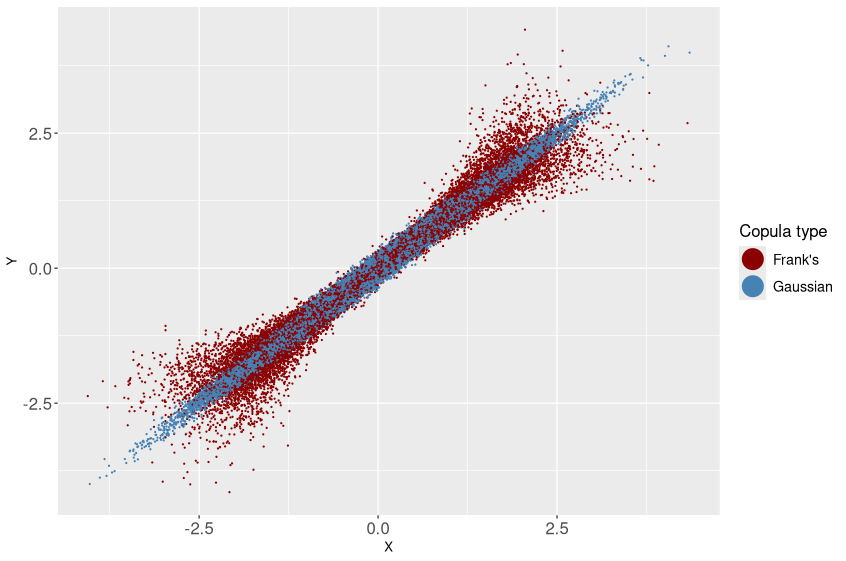
\includegraphics[width=0.7\linewidth]{CopulaVergelijking.png}
    \caption{Different copulas for lognormal marginals with the same correlation coefficient}
    \label{fig:copulavergelijking}
\end{figure}

\begin{comment}
\begin{figure}[h]
\begin{subfigure}{0.47\textwidth}
    \centering
    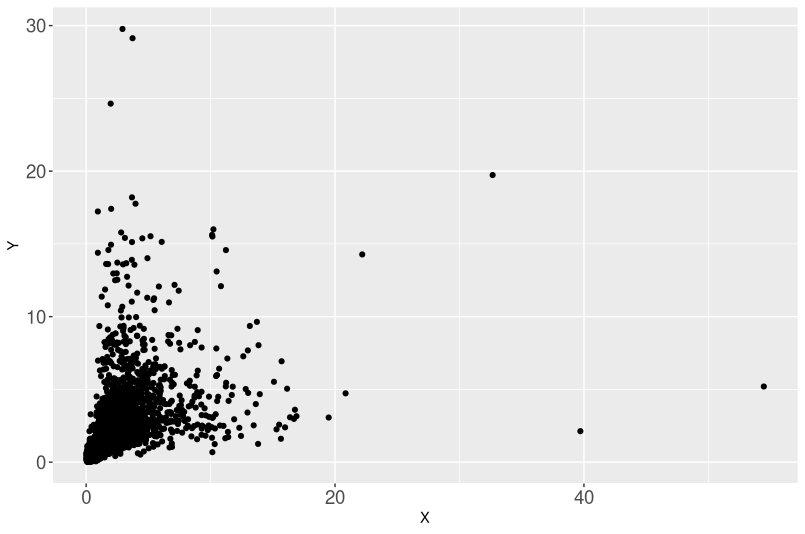
\includegraphics[width=\linewidth]{Frank's copula.png}
    \caption{Frank's copula for lognormal marginals}
    \label{fig:Frank's copula}
\end{subfigure}
\hfill
\begin{subfigure}{0.47\textwidth}
    \centering
    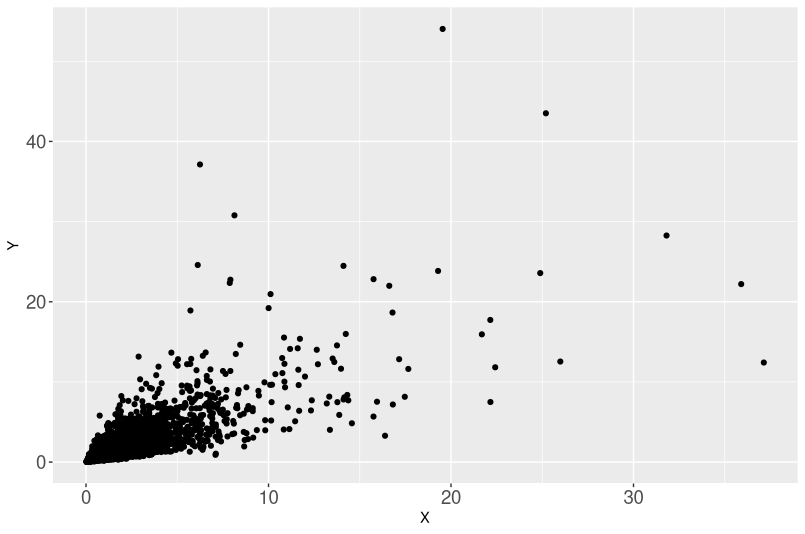
\includegraphics[width=\linewidth]{Gaussian copula.png}
    \caption{Gaussian copula for lognormal marginals}
    \label{fig:Gaussian copula}
\end{subfigure}
\caption{Different copulas for lognormal marginals with same correlation coefficient}
\end{figure}
\end{comment}

\begin{comment}
We can use the second part of Theorem \ref{Sklar's theorem} to take a look at the dependence structure of two logistically distributed random variables when assuming different underlying copulas. In Figure \ref{fig:Frank's copula} we see the correlation between two logistically distributed random variables with an underlying Frank's copula with $\alpha = 0.7$. We can now compare this to Figure \ref{fig:Gaussian copula} where the underlying copula is the Gaussian copula with parameter $\alpha = 0.7$.
\begin{figure}[h]
\begin{subfigure}{0.47\textwidth}
    \centering
    \includegraphics[width=\linewidth]{Frank_copula.png}
    \caption{Frank's copula for logistic marginals}
    \label{fig:Frank's copula}
\end{subfigure}
\hfill
\begin{subfigure}{0.47\textwidth}
    \centering
    \includegraphics[width=\linewidth]{Gaussian_copula.png}
    \caption{Gaussian copula for logistic marginals}
    \label{fig:Gaussian copula}
\end{subfigure}
\caption{Different copulas for logistic marginals}
\end{figure}
\end{comment}

\section{Aggregate risk of lognormal variables under a Gaussian copula model}

We say that a random variable $X$ is distributed lognormally if the logarithm of $X$ follows a normal distribution.
In financial mathematics, this is one of the most popular distributions used in modelling stock prices and, more relevant to our `case study', insurance claims. 

Assume the insurer takes on $n$ individual risks. Denote $X_i$ as the (positive) random variable that represents the amount the insurer has to pay to policyholder $i$. Let $w_i > 0$ represent the weight of the risk $X_i$. The aggregate loss of the insurer is given as
$$S = \sum_{i=1}^nw_iX_i.$$
For now we will assume that each $X_i$ follows a lognormal distribution: $X_i\sim \text{Lognormal}(1,0)$. We wish to study the behaviour of $S$, therefore we will begin with some initial simulations to get a sense of how $S$ is distributed.

Suppose that $n  = 100$, the insurer takes on $100$ individual risks $X_1,X_2,\dots,X_{100}$ with $X_i\sim \text{Lognormal}(0,1)$ and $w_i = 1$ for every $i\in \{1,2,\dots,n\}$. Thus $S = \sum_{i=1}^nX_i$. In addition we assume that the underlying copula is a Gaussian copula with correlation matrix $\Sigma$ such that $\Sigma_{ij} = \rho = 0.7$ if $i\neq j$ and $\Sigma_{ii} = 1$. The joint cumulative distribution function of the random vector $(X_1,X_2,\dots,X_n)$ is given as in Theorem \ref{Sklar's theorem 2.0} for the copula in Definition \ref{def: Gaussian copula}. We simulate the aggregate loss by taking multiple samples from the joint distribution of this random vector. Figure \ref{fig:aggregate_loss} shows the result of this process for a sample size of $10000$. 
%We will take a look at the impact of the choice of copula on the distribution of the aggregate loss. \\\\
%Let us look at the case where the insurer takes on $100$ individual risks ($n = 100$),  $X_i\sim \text{Lognormal}(0,1)$ and $w_i = 1$ for every $i$. We first assume a Frank's copula with parameter $\alpha = 10$, simulating the aggregate loss for a sample size of 10000, we find results as shown in Figure \ref{fig:aggregate loss frank}. Again making sure that the correlation matrix is (approximately) the same as for the sample with Frank's copula, Figure \ref{fig:aggregate loss gaussian} shows a sample distribution with a Gaussian copula. We can now calculate the Value-at-Risk and the Tail Value-at-Risk for $p = 0.99$ for both cases. Assuming a Frank's copula we find $\text{VaR} = 724.13$ and $\text{TVaR} = 829.13$. Assuming a Gaussian copula we find $\text{VaR} = 875.01$ and $\text{TVaR} = 1218.04$. So we notice a significant difference between the respective values at risk and tail values at risk. So depending on the estimation of the copula, the perspective and the actions of the insurer should vary.
\begin{comment}
\begin{figure}[h]
\begin{subfigure}{0.47\textwidth}
    \centering
    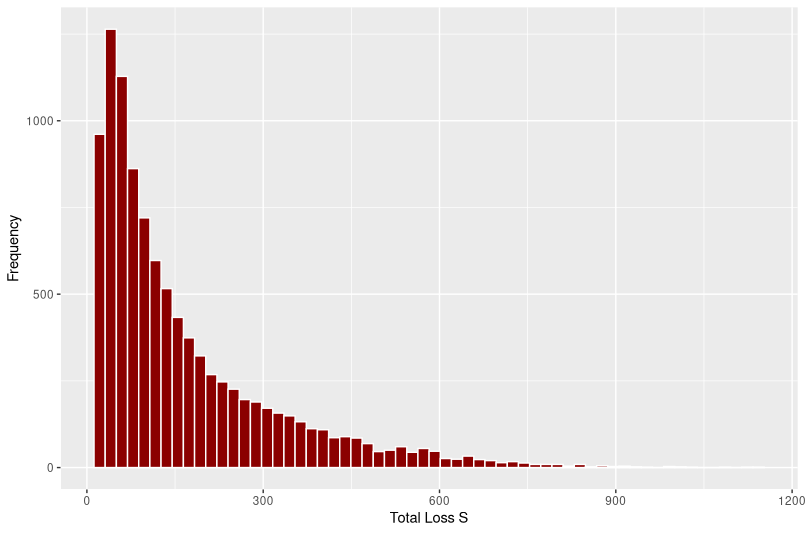
\includegraphics[width=\linewidth]{aggregate_loss_frank.png}
    \caption{Aggregate loss with Frank's copula}
    \label{fig:aggregate loss frank}
\end{subfigure}
\hfill
\begin{subfigure}{0.47\textwidth}
    \centering
    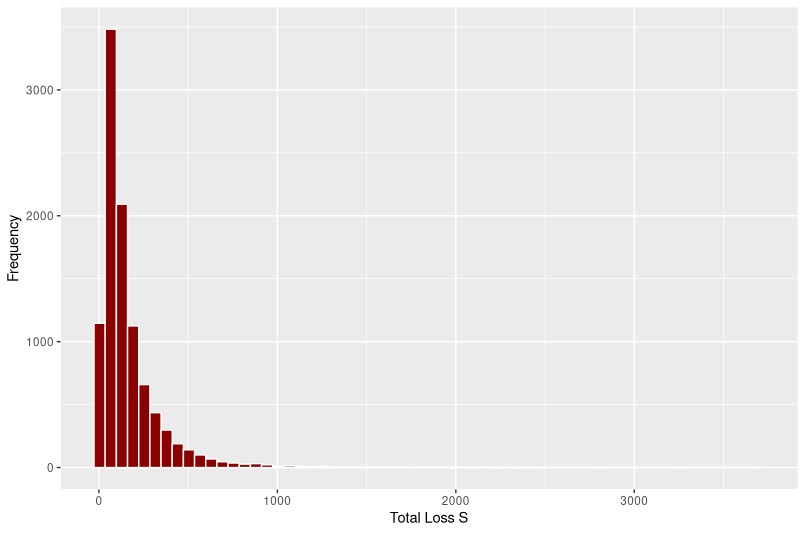
\includegraphics[width=\linewidth]{aggregate_loss_gaussian.png}
    \caption{Aggregate loss with Gaussian copula}
    \label{fig:aggregate loss gaussian}
\end{subfigure}
\caption{Aggregate loss distributions for different copulas}
\end{figure}
\end{comment}
% In addition we assume that Corr$(X_i,X_j) = 0.7$ for every $i,j\in \{1,\dots,n\}$ with $i\neq j$. Figure \ref{fig:aggregate_loss} shows the distribution of $S$ for a sample size of $10000$.
\begin{figure}[h!]
    \centering
    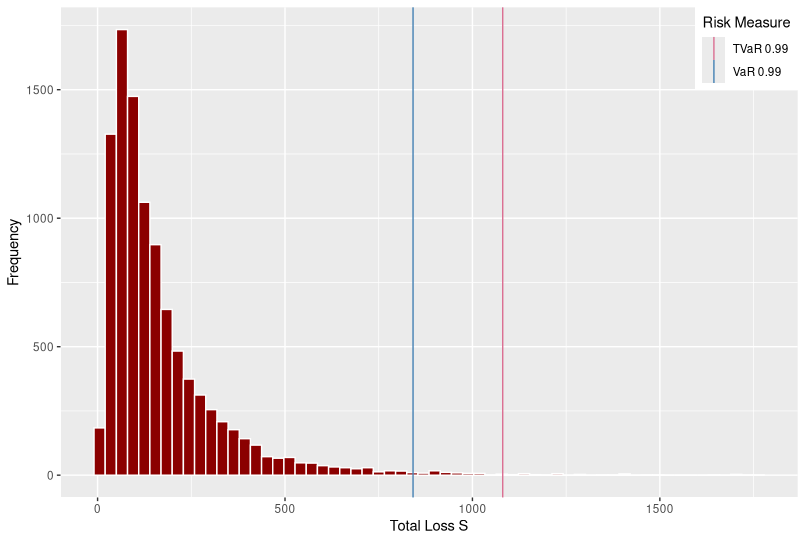
\includegraphics[width=0.7\linewidth]{Aggregate_loss_0.7.png}
    \caption{Aggregate loss for $n = 100$ and $\rho = 0.7$}
    \label{fig:aggregate_loss}
\end{figure}

% Deze waarden toevoegen aan grafiek als rechten
\begin{figure}[h]
\begin{subfigure}{0.47\textwidth}
    \centering
    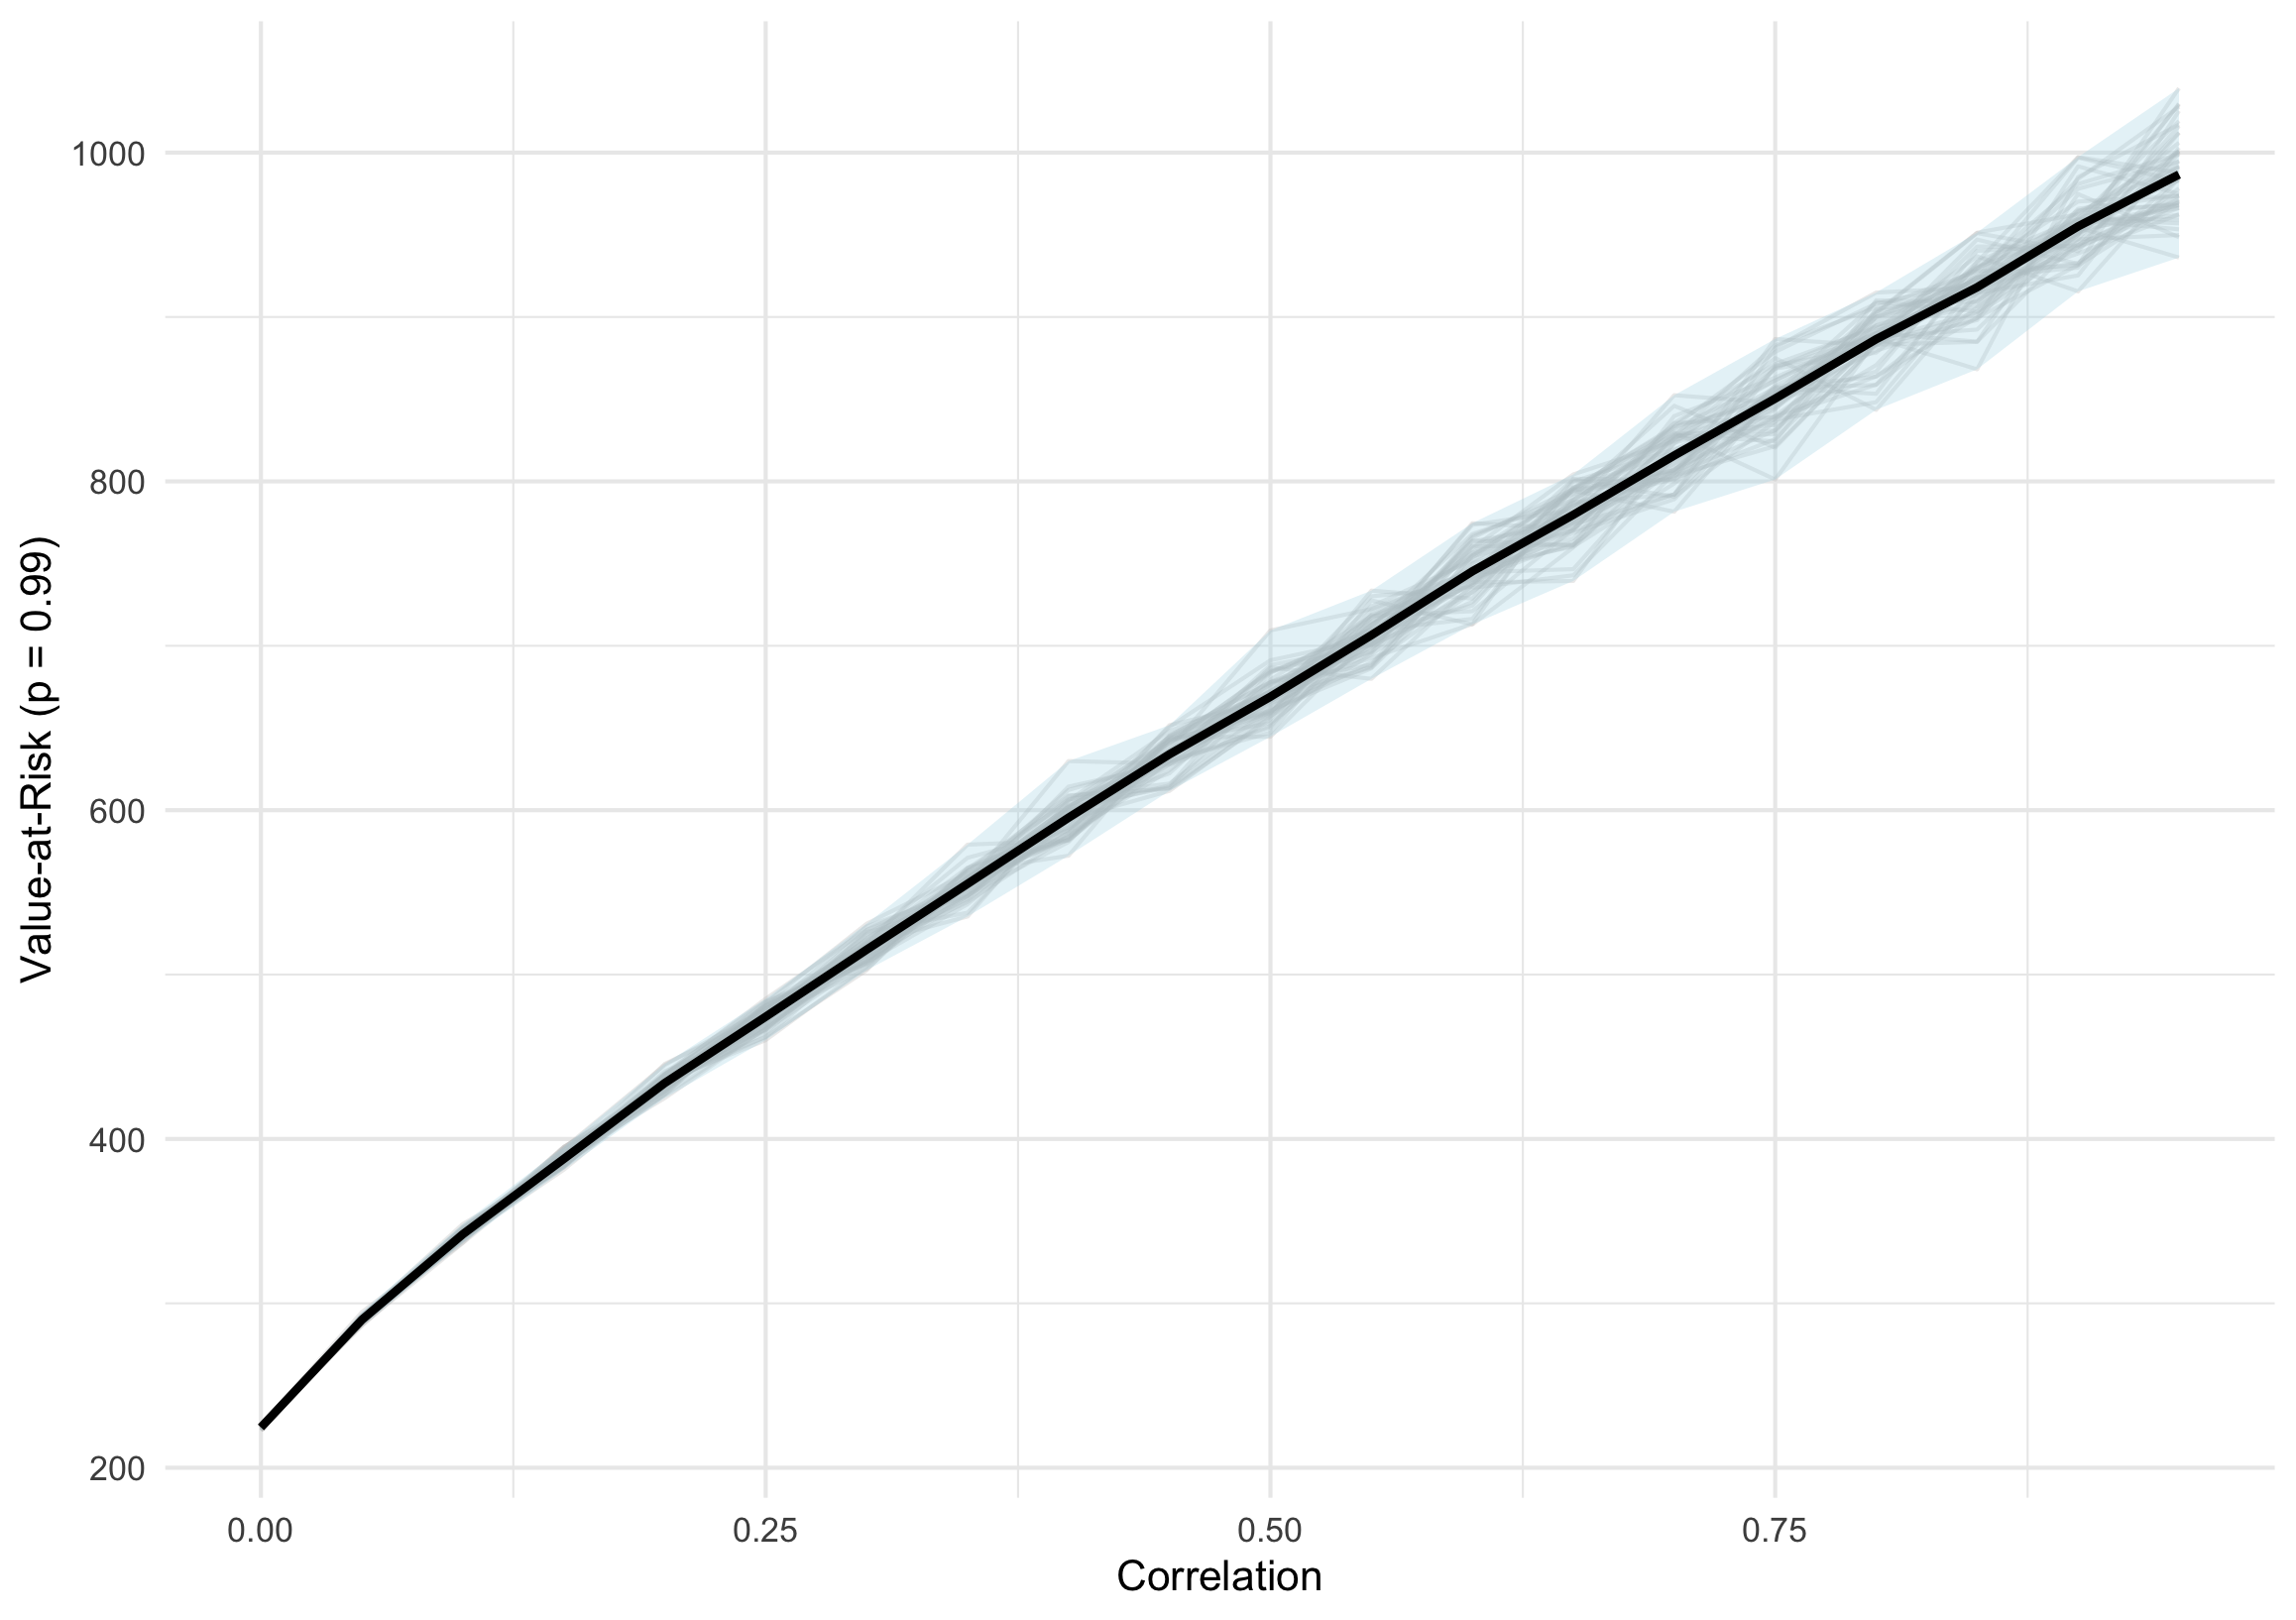
\includegraphics[width=\linewidth]{VaR-band.png}
    \caption{Value-at-Risk}
    \label{fig:VaR}
\end{subfigure}
\hfill
\begin{subfigure}{0.47\textwidth}
    \centering
    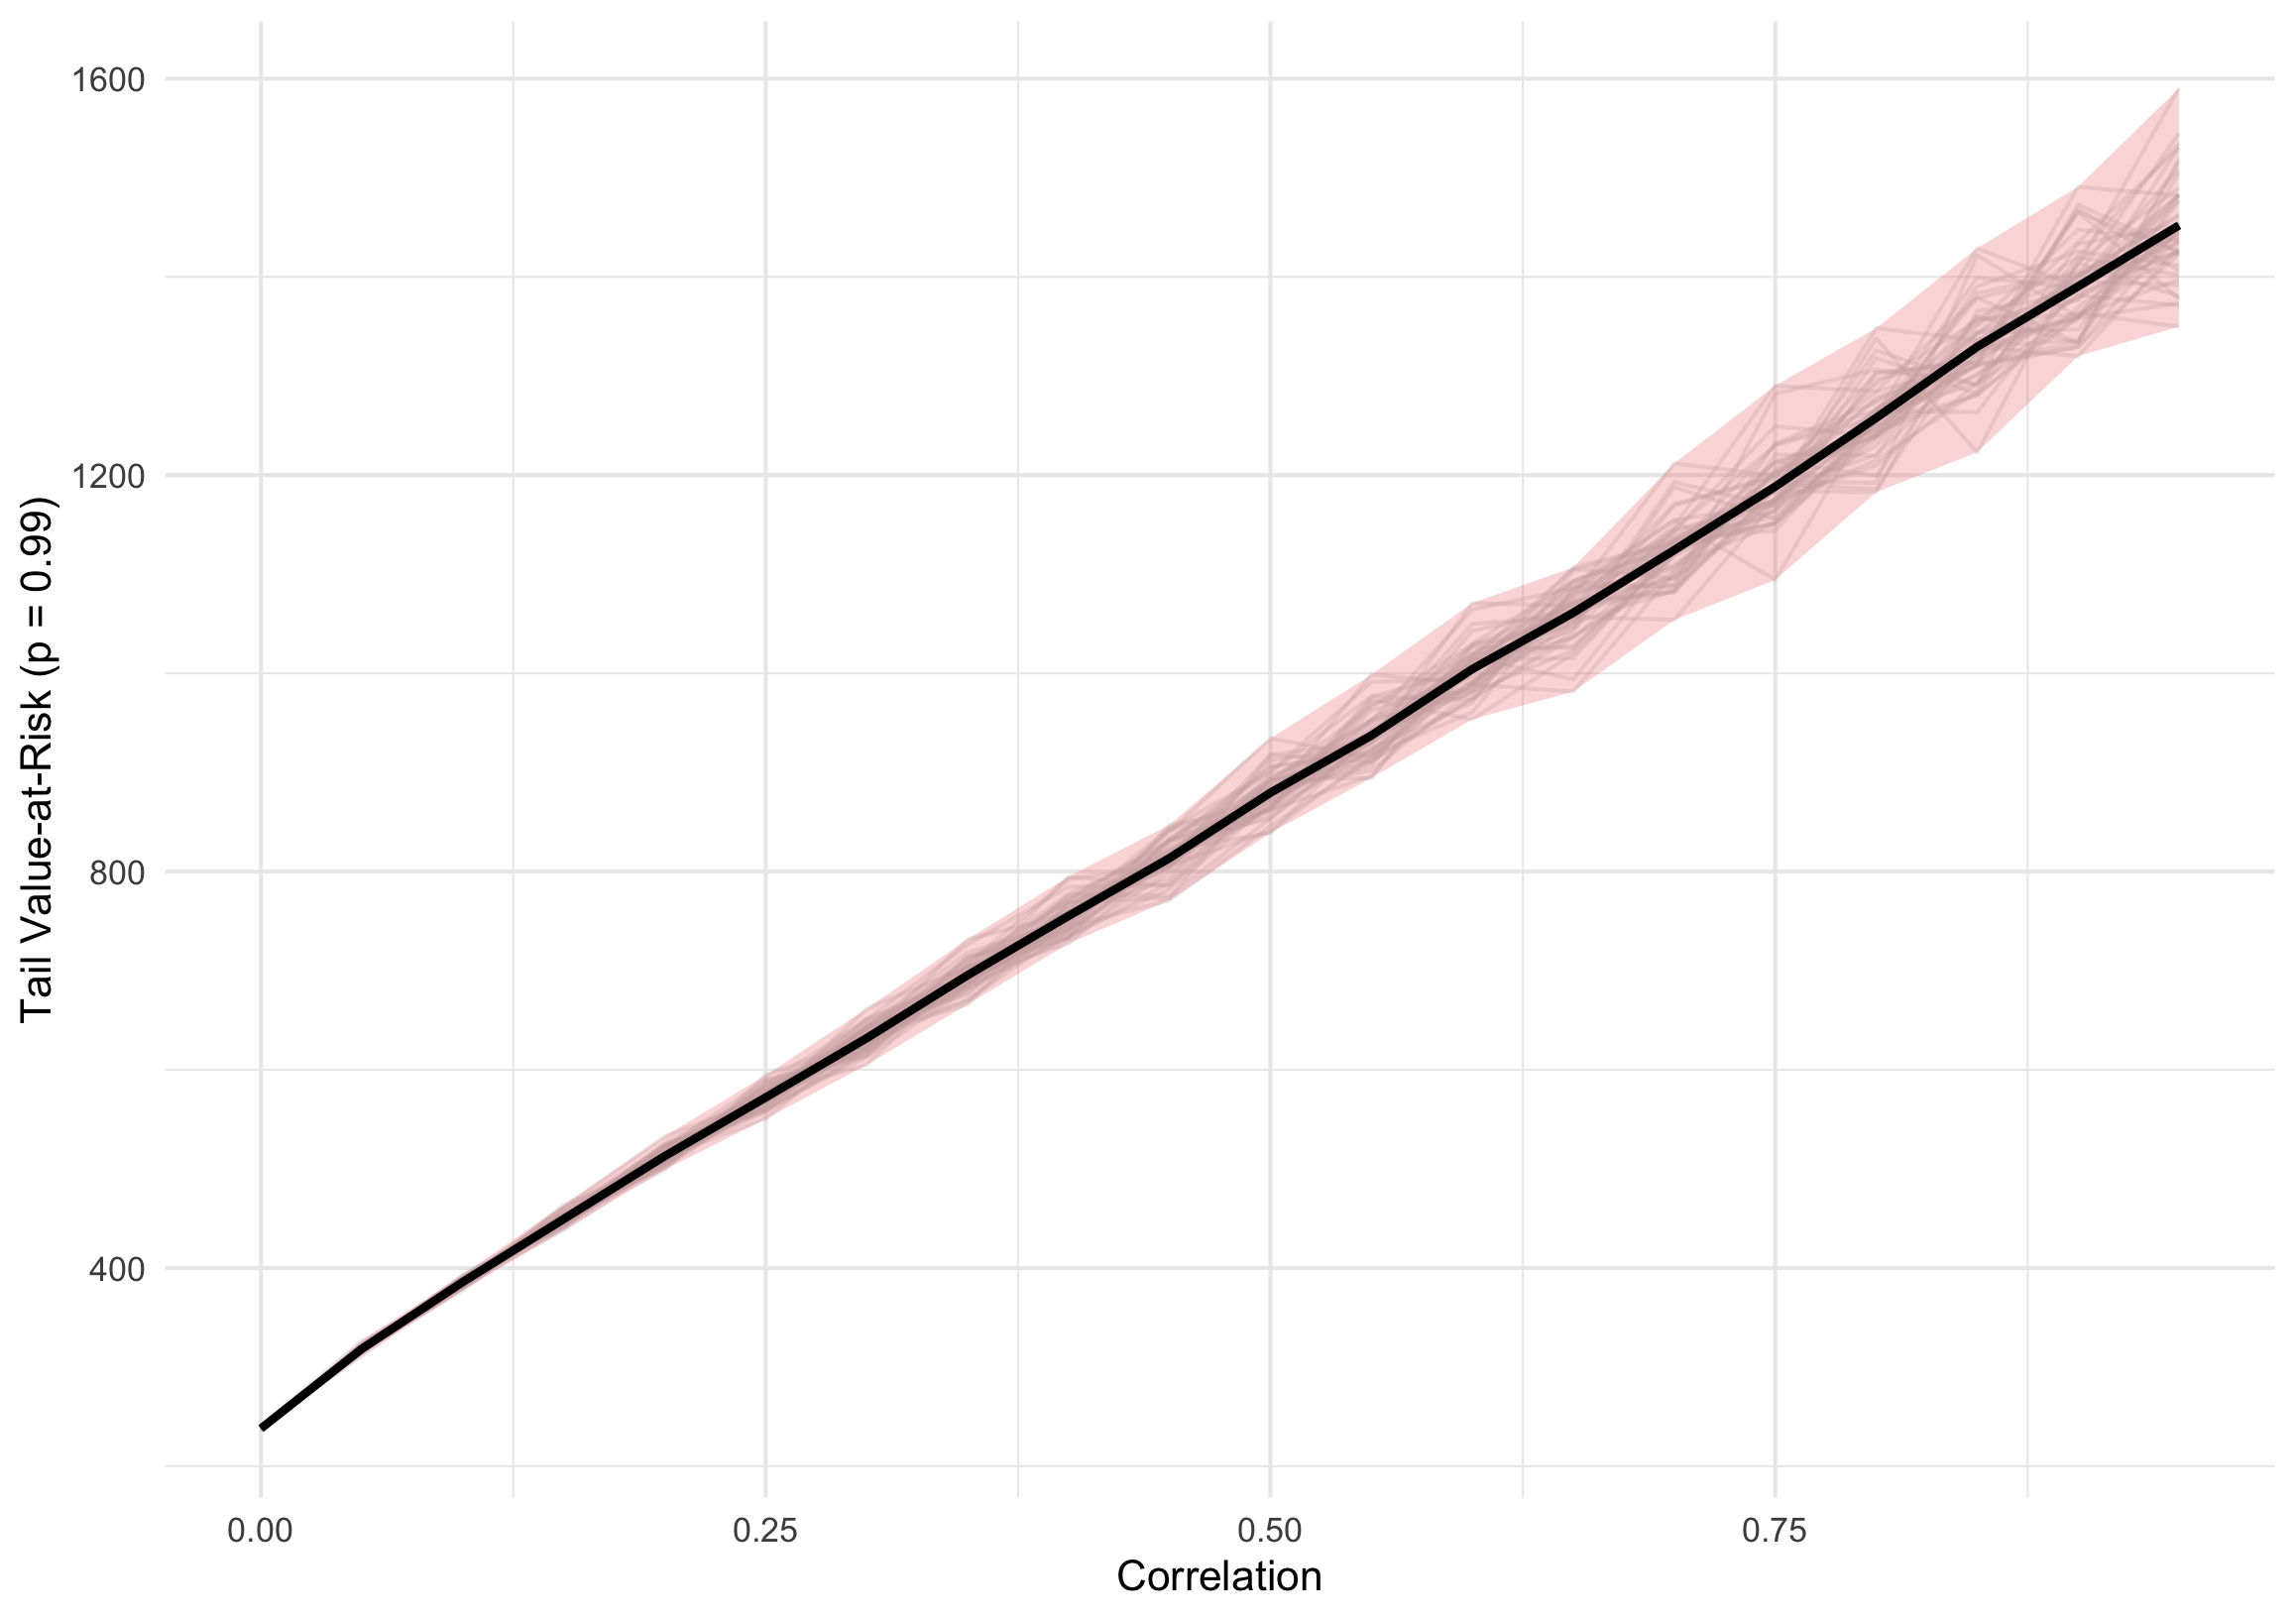
\includegraphics[width=\linewidth]{TVaR-band.png}
    \caption{Tail Value-at-Risk}
    \label{fig:TVaR}
\end{subfigure}
\caption{Risk measures as functions of the correlation}
\end{figure}

We can now study the influence of the correlation coefficient on the Value-at-Risk and the Tail Value-at-Risk. Here we will still assume that Corr$(X_i,X_j) = \rho$ does not depend on $i,j\in \{1,\dots, n\}$  (and varies from 0 to 0.99) if $i\neq j$ and that $X_i\sim \text{Lognormal}(0,1)$ for every $i\in \{1,\dots,n\}$. Again, we take $n = 100$ and will use a sample size of $25000$. Figure \ref{fig:VaR} shows the calculated Value-at-Risk for the different correlation coefficients $\rho$ and Figure \ref{fig:TVaR} shows the calculated Tail Value-at-Risk for the different correlation coefficients $\rho$. The Monte Carlo experiment was repeated $50$ times: the coloured bands indicate the range of observed outcomes, the thin gray lines represent individual repetitions and the thick black line is the mean of all repetitions.

The key takeaway here is that both the Value-at-Risk and Tail Value-at-Risk are approximately linear in the correlation, and intuitively this makes a lot of sense: if there is a lot of dependence between the individual variables, the chance increases that they all ``fail together'', that is to say: the fact that the losses move in lock-step is precisely what it \textit{means} for the variables to be correlated.

In attempting a more analytical approach to learning more about $S$, one quickly finds out a rather unfortunate fact: \textit{there is no closed formula for the distribution of a sum of lognormals}. This means that we will have to rely on approximations for this sum in order to say anything relevant about it. We will do this by searching for upper and lower bounds on $S$, so as to at least find a band in which the sum will certainly lie. The attentive reader will have noticed that there is a priori no single way to compare two random variables, and as such it is not well-defined to talk about bounds. In the next section, we will define several ways to define an ordering on random variables, and use such a system to bound the aggregate risk.

\section{Ordering of random variables}
In order to determine upper and lower bounds for the aggregate risk, we first have to define an ordering system for random variables. There are multiple ways to construct an ordering on random variables. From this section on we will assume that all functions are differentiable with absolutely continuous derivative.
\begin{definition}\cite[Definition 1.6.1]{Risk_Measurement}
    Suppose $A\subseteq \mathbb{R}$ an interval and $u: A\rightarrow A$ a function. $u$ is said to be concave if for every $x,y\in A$ and every $t\in [0,1]$, it holds that
    $$u(t \cdot x + (t-1) \cdot y) \geq t \cdot u(x) + (t-1) \cdot u(y).$$
    A function $v : A \rightarrow A$ is said to be convex if $(-v)$ is concave.
\end{definition}
\begin{definition}[\textbf{Stop-loss premium}]\cite[Definition 2.3.2]{Risk_Measurement}
   The stop-loss premium with retention $K\in \mathbb{R}$ of a random variable $X$ is given by $\mathbb{E}[(X-K)_+]$.
\end{definition}
Here we use the notation $(x-K)_+ = \max\{x-K,0\}$ for $x\in \mathbb{R}$. The value $\mathbb{E}[(X-K)_+]$ corresponds to the surface between the cumulative distribution function $F_X$ of $X$ and the constant function $1$ from $K$ on. This means that we can interpret the stop-loss premium with retention $K$ of $X$ as the weight of the upper tail of $X$. Hence, a larger stop-loss premium indicates that the loss can be considered more dangerous, since the probability of large claims is higher.
\begin{definition}[\textbf{Convex order}]\cite[Definition 2.5.1]{Risk_Measurement}
    Consider two random variables $X$ and $Y$. We say that $X$ precedes $Y$ in convex order sense, if 
    $$\mathbb{E}[X] = \mathbb{E}[Y]$$
    and 
    $$\mathbb{E}[u(-X)] \geq \mathbb{E}[u(-Y)]$$
    for all non-decreasing concave functions $u$ for which the expectation exists. We write $X\preceq_{cx}Y$.
\end{definition}

Convex order is an interesting concept to consider. In the expected utility framework, concave utility functions correspond to risk-averse agents: so if $X \preceq_{cx} Y$, then $X$ is preferred to $Y$ by every possible risk-averse agent. It arises naturally when considering \textit{stop-loss ordering}, i.e. the same ordering as convex ordering, but relaxing the condition of equality of $\mathbb{E}[X]$ and $\mathbb{E}[Y]$. Indeed, we use stop-loss ordering to replace a potentially complicated loss $X$ with a more sizeable risk $Y$, which might have an easier distribution. Then it stands to reason that the best approximations for $X$ are those where we already match the expected value.

\begin{lemma}\cite[Lemma 2.6.1]{Risk_Measurement}\cite[Lemma 1]{cheung-2013}\label{lemma: integral representation}
    Suppose $X$ a random variable with finite expectation and cumulative distribution function $F$. Assume that $I\subseteq \mathbb{R}$ an interval such that $F:I \rightarrow (0,1)$ is bijective. Let $f: I \rightarrow \mathbb{R}$ a convex function with absolutely continuous derivative $f'$. If $a\in I$, then 
    \begin{equation}\label{vgl: expectation integral representation}
    \mathbb{E}[f(X)] = f(a) + f'(a)\;(\mathbb{E}[X] - a) + \int_{\inf I}^af''(K)\;\mathbb{E}[(K-X)_+]dK + \int^{\sup I}_af''(K)\;\mathbb{E}[(X-K)_+]dK.
    \end{equation}
\end{lemma}
\begin{proof}
    We will start by proving 
    \begin{equation}\label{vgl: integral representation}
        f(x) = f(a) + f'(a)(x-a) + \int_{\inf I}^af''(K)\;(K-x)_+dK + \int^{\sup I}_af''(K)\;(x-K)_+dK
    \end{equation}
    for every $x\in I$. Suppose $x\in I$. Since $f'$ is absolutely continuous, $f$ must also be absolutely continuous. Hence
    $$f(x) = f(a) - \int_x^af'(K)dK.$$
    By partial integration we find
    $$f(x) = f(a) - af'(a)+xf'(x) + \int_x^af''(K)\;K\;dK.$$
    If $a \leq x$, we have
    \begin{align*}
    xf'(x) + \int_x^af''(K)\;K\;dK &= \int_a^xf''(K)(x-K)dK\\
    &= \int^{\sup I}_af''(K)\;(x-K)_+dK\\
    &= \int_{\inf I}^af''(K)\;(K-x)_+dK + \int^{\sup I}_af''(K)\;(x-K)_+dK,
    \end{align*}
    since $(K-x)_+ = 0$ for $K \in (\inf I, a)$. Analogously, if $a> x$ we find
    \begin{align*}
    xf'(x) + \int_x^af''(K)\;K\;dK &= \int_x^af''(K)(K-x)dK\\
    &= \int_{\inf I}^af''(K)\;(K-x)_+dK\\
    &= \int_{\inf I}^af''(K)\;(K-x)_+dK + \int^{\sup I}_af''(K)\;(x-K)_+dK,
    \end{align*}
    where we used that $(x-K)_+ = 0$ for $K \in (a, \sup I)$. We have proven that \eqref{vgl: integral representation} holds for every $x\in \mathbb{R}$. By replacing $x$ with the random variable $X$ we have
    \begin{equation}
        f(X) = f(a) + f'(a)(X-a) + \int_{\inf I}^af''(K)\;(K-X)_+dK + \int^{\sup I}_af''(K)\;(X-K)_+dK.
    \end{equation}
    By taking the expectation of both sides we find
    $$\mathbb{E}[f(X)] = f(a) + f'(a)\;(\mathbb{E}[X] - a) + \mathbb{E}\left[\int_{\inf I}^af''(K)\;(K-X)_+dK + \int^{\sup I}_af''(K)\;(X-K)_+dK\right]. $$
    Notice that the functions in the integral are all positive definite, hence we can apply Fubini's Theorem and conclude that \eqref{vgl: expectation integral representation} holds.
\end{proof}
\begin{theorem} \cite[Section 3.A.1]{shaked-2007}\label{equivalent definitions cx}
    Let $X,Y$ be random variables. The following are equivalent
    \begin{enumerate}
        \item $ X\preceq_{cx}Y$,
        \item $\mathbb{E}[X] = \mathbb{E}[Y]$ and $\mathbb{E}[(X-K)_+] \leq \mathbb{E}[(Y-K)_+]$ for all $K\in \mathbb{R}$,
        \item $\mathbb{E}[X] = \mathbb{E}[Y]$ and $\mathbb{E}[(K-X)_+] \leq \mathbb{E}[(K-Y)_+]$ for all $K\in \mathbb{R}$,
        \item $\mathbb{E}[v(X)] \leq \mathbb{E}[v(Y)]$ for all convex functions $v$ for which the expectations exist.
    \end{enumerate}
\end{theorem}
\begin{proof}
\textbf{1. $\Rightarrow$ 2.} Suppose $X\preceq_{cx} Y$ and choose $K\in \mathbb{R}$. $x\mapsto -x$ and $x\mapsto (x-K)_+$ are two convex functions, hence $x\mapsto (-x-K)_+$ is also convex. In addition we have that this function is non-increasing. It follows that $u: \mathbb{R}\rightarrow \mathbb{R}: x\mapsto -(-x-K)_+$ is a non-decreasing concave function. Thus $\mathbb{E}[u(-X)] \geq \mathbb{E}[u(-Y)]$, and
$$\mathbb{E}[-(X - K)_+] \geq \mathbb{E}[-(Y-K)_+].$$
Hence we can conclude that
$$\mathbb{E}[(X - K)_+] \leq \mathbb{E}[(Y-K)_+]$$
for all $K\in \mathbb{R}$.
\\\\
\textbf{2. $\iff$ 3.} If $K\in \mathbb{R}$, we know that 
\begin{align*}
    \mathbb{E}[(X-K)_+] -\mathbb{E}[(K-X)_+] &= \mathbb{E}[\max\{0,X-K\}] - \mathbb{E}[\max\{0,K-X\}]\\
    &= \mathbb{E}[X-K] \\
    &= \mathbb{E}[X] - K.
\end{align*}
Thus if $\mathbb{E}[X] = \mathbb{E}[Y]$, we have
$$\mathbb{E}[(X-K)_+] \leq \mathbb{E}[(Y-K)_+]$$
if and only if
$$\mathbb{E}[(K-X)_+] + \mathbb{E}[X] - K \leq \mathbb{E}[(K-Y)_+] + \mathbb{E}[Y] - K,$$
which is equivalent with 
$$\mathbb{E}[(K-X)_+] \leq \mathbb{E}[(K-Y)_+].$$

\textbf{4. $\Rightarrow$ 1.} Suppose that $\mathbb{E}[v(X)] \leq \mathbb{E}[v(Y)]$ for all convex functions $v$ for which the expectations exist. Let $u: \mathbb{R}\rightarrow \mathbb{R}$ be a non-decreasing concave function. Then it holds that $v:\mathbb{R}\rightarrow\mathbb{R}: x\mapsto -u(-x)$ is a convex function. Thus 
$$\mathbb{E}[v(X)]\leq \mathbb{E}[v(Y)].$$
Hence we conclude that
$$\mathbb{E}[u(-X)]\geq \mathbb{E}[u(-Y)].$$
\\\\
\textbf{3. $\Rightarrow$ 4.} Suppose that $\mathbb{E}[X] = \mathbb{E}[Y]$ and $\mathbb{E}[(K-X)_+] \leq \mathbb{E}[(K-Y)_+]$ for all $K\in \mathbb{R}$. We have already proven that this also means that $\mathbb{E}[(X-K)_+] \leq \mathbb{E}[(Y-K)_+]$ for all $K\in \mathbb{R}$. Suppose that $v:\mathbb{R}\rightarrow \mathbb{R}$ is a convex function for which the expectations exist. Applying Lemma \ref{lemma: integral representation} for $a = \mathbb{E}[X] = \mathbb{E}[Y]$ we have
\begin{align*}
\mathbb{E}[v(X)] &= v(\mathbb{E}[X]) + v'(\mathbb{E}[X])\;(\mathbb{E}[X] - \mathbb{E}[X]) + \int_{-\infty}^{\mathbb{E}[X]}v''(K)\;\mathbb{E}[(K-X)_+]dK \\
&\quad\quad+ \int^{\infty}_{\mathbb{E}[X]}v''(K)\;\mathbb{E}[(X-K)_+]dK\\
&= v(\mathbb{E}[X])+ \int_{-\infty}^{\mathbb{E}[X]}v''(K)\;\mathbb{E}[(K-X)_+]dK + \int^{\infty}_{\mathbb{E}[X]}v''(K)\;\mathbb{E}[(X-K)_+]dK.
\end{align*}
Since $v$ is a convex function with second derivative $v''$, it holds that $v''(x) \geq 0$ for every $x\in \mathbb{R}$. Thus by our initial assumption, it holds that 
$$v''(K)\;\mathbb{E}[(X-K)_+] \leq v''(K)\;\mathbb{E}[(Y-K)_+]$$
and 
$$v''(K)\;\mathbb{E}[(K-X)_+] \leq v''(K)\;\mathbb{E}[(K-Y)_+]$$
for all $K\in \mathbb{R}$. Thus since $\mathbb{E}[X] = \mathbb{E}[Y]$, it follows that
\begin{align*}
    \mathbb{E}[v(X)] &= v(\mathbb{E}[Y])+ \int_{-\infty}^{\mathbb{E}[Y]}v''(K)\;\mathbb{E}[(K-X)_+]dK + \int^{\infty}_{\mathbb{E}[Y]}v''(K)\;\mathbb{E}[(X-K)_+]dK\\
    &\leq v(\mathbb{E}[Y])+ \int_{-\infty}^{\mathbb{E}[Y]}v''(K)\;\mathbb{E}[(K-Y)_+]dK + \int^{\infty}_{\mathbb{E}[Y]}v''(K)\;\mathbb{E}[(Y-K)_+]dK\\
    &= \mathbb{E}[v(Y)].
\end{align*}
\end{proof}

\begin{proposition}\label{prop: inequality of variances convex order}
    If $X$ and $Y$ are random variables such that $X\preceq_{cx} Y$, then $\text{Var}[X]\leq \text{Var}[Y]$.
\end{proposition}
\begin{proof}
    $x\mapsto x^2$ is a convex function, thus it follows from Theorem \ref{equivalent definitions cx} that $\mathbb{E}[X^2] \leq \mathbb{E}[Y^2]$. Since $\mathbb{E}[X] = \mathbb{E}[Y]$, we see that $\text{Var}[X]\leq \text{Var}[Y]$.
\end{proof}

\begin{proposition}\cite[Theorem 6.5.2]{Risk_Measurement}\label{prop: tvar consistent with convex order}
    For random variables $X,Y$ with $X\preceq_{cx}Y$ it holds that $\text{TVaR}_p[X]\leq \text{TVaR}_p[Y] $ for every $p\in (0,1)$.
\end{proposition}
% Door dit bewijs zou sectie 7.3.4 Tail Value-at-Risk wat ingekort kunnen worden omdat daar een analoge redenering gebruikt wordt.
\begin{proof}
    Suppose $p\in (0,1)$. Then for $U\sim \text{Uniform}(0,1)$ it holds
    \begin{align*}
        \text{TVaR}_p[X] &= \frac{1}{1-p} \int_p^1F_X^{-1}(q)\;dq\\
        &= \frac{1}{1-p} \mathbb{E}\left[F_X^{-1}(U)\;\mathbbm{1}_{U > p}\right]\\
        &= \frac{1}{1-p} \mathbb{E}\left[F_X^{-1}(U)\;\mathbbm{1}_{F_X^{-1}(U) > F_X^{-1}(p)}\right] \\
        &= \frac{1}{1-p} \mathbb{E}\left[X\;\mathbbm{1}_{X > F_X^{-1}(p)}\right].
    \end{align*}
    Analogously we find 
    $$ \text{TVaR}_p[Y] = \frac{1}{1-p} \mathbb{E}\left[Y\;\mathbbm{1}_{Y > F_Y^{-1}(p)}\right].$$
    By Theorem \ref{equivalent definitions cx} we know that $\mathbb{E}[v(X)]\leq \mathbb{E}[v(Y)]$ for all convex functions $v$ for which these expectations exist. We know that 
    $$\mathbb{R}\rightarrow \mathbb{R}:x\mapsto x\;\mathbbm{1}_{x>d}(x)$$
    is convex for every $d\in \mathbb{R}$. Thus we can conclude that
    $$\text{TVaR}_p[X] = \frac{1}{1-p} \mathbb{E}\left[X\;\mathbbm{1}_{X > F_X^{-1}(p)}\right]\leq \frac{1}{1-p} \mathbb{E}\left[Y\;\mathbbm{1}_{Y > F_Y^{-1}(p)}\right]  = \text{TVaR}_p[Y].$$
\end{proof}

Having defined a reasonable interpretation for ordering random variables, we can start to use properties of this ordering to find lower and upper bounds for the aggregate risk of lognormals with a Gaussian copula. Note that it is mainly the lower bound which is of interest to an insurer: the end goal is still to gain an idea of how much money to put aside, and since the scenario in which we turn out not to have enough solvency capital is very much to be avoided, this will provide us with a \textit{minimum minimorum} to put aside.

\section{Upper and lower bounds for the aggregate risk}\label{section: upper and lower bounds}
Assuming we know the marginal distributions of the individual risks and the relevant copula, we are interested in the properties of the distribution of $$S = \sum_{i=1}^n X_i.$$ In our case we will assume that the individual risks each follow a lognormal distribution and that the underlying copula is a Gaussian copula. Since there is no closed formula for the distribution of $S$ we have to investigate other methods to study the behaviour of the aggregate risk. One way to do this is to search for upper and lower bounds. So we want random variables $S^u$ and $S^l$ such that 
$$ S^l \preceq_{cx} S \preceq_{cx} S^u.$$
\subsection{Upper bounds}
Suppose that $F_1,F_2,\dots, F_n$ are the marginal cumulative distribution functions of the random variables $X_1,X_2,\dots,X_n$. Let $(a_i,b_i)\subseteq\mathbb{R}$ such that $F_i: (a_i,b_i)\rightarrow(0,1)$ is a continuous bijection. Define $S^u := F^{-1}_1(U) + F^{-1}_2(U) + \dots + F^{-1}_n(U)$ where $U$ is a uniformly distributed random variable over $(0,1)$. 
\begin{lemma}\cite[Theorem 3.2.2]{Risk_Measurement}\label{inverse distribution function h(X)}
    Suppose that $X$ is a random variable with cumulative distribution function $F_X : (a,b)\rightarrow (0,1)$ (here we do not require $F_X$ to be continuous). Let $h : (a,b) \rightarrow \mathbb{R}$ be a non-decreasing, left-continuous function. Then the following holds:
    $$F_{h(X)}^{-1}(p) = h(F_X^{-1}(p))$$
    for all $p\in (0,1)$.
\end{lemma}
\begin{proof}
    Suppose $p\in (0,1)$. If $F: I\subseteq\mathbb{R}\rightarrow (0,1)$ is a cumulative distribution function, $x\in I$ and $q\in(0,1)$ it holds that
    \begin{equation}\label{property cdf}
        F^{-1}(q) \leq x \iff q \leq F(x).
    \end{equation}
    $h$ is non-decreasing and left-continuous, which means that 
    $$h(z) \leq x\iff z\leq \sup\{y\mid h(y)\leq x\}$$
    for every $x\in \mathbb{R}$ and $z\in (a,b)$. Thus we find
    \begin{align*}
        F_{h(X)}^{-1} \leq x &\iff p \leq F_{h(X)}(x) \\
        &\iff p \leq P[h(X)\leq x]\\
        &\iff p \leq P[X\leq \sup\{y\mid h(y)\leq x\}]\\
        &\iff p \leq F_X( \sup\{y\mid h(y)\leq x\}).
    \end{align*}
    We claim that 
    \begin{equation}\label{equivalence of probabilities}
        p \leq F_X( \sup\{y\mid h(y)\leq x\}) \iff F_X^{-1}(p) \leq  \sup\{y\mid h(y)\leq x\}.
    \end{equation}
    By Property \ref{property cdf} this is true if $ \sup\{y\mid h(y)\leq x\}$ is finite. If $ \sup\{y\mid h(y)\leq x\} = -\infty$ we see that $p \leq 0\iff F_X^{-1}(p)\leq -\infty$ indeed holds. For $ \sup\{y\mid h(y)\leq x\} = \infty$ we see that $p \leq 1\iff F_X^{-1}(p)\leq \infty$ is also true. Hence we can conclude that the equivalence \eqref{equivalence of probabilities} holds. We found that
    \begin{equation*}
        F_{h(X)}^{-1}(p) \leq x \iff F_X^{-1}(p) \leq  \sup\{y\mid h(y)\leq x\}.
    \end{equation*}
    $h$ is non-decreasing and left continuous, hence
    $$F_X^{-1}(p) \leq  \sup\{y\mid h(y)\leq x\} \iff h(F_X^{-1}) \leq x.$$
    Thus 
    $$F_{h(X)}^{-1}(p) \leq x  \iff h(F_X^{-1}) \leq x$$
    holds for every $x$. We conclude that $F_{h(X)}^{-1}(p) = h(F_X^{-1}(p))$.
\end{proof}
\begin{proposition}\cite[Theorem 4.1.1]{Risk_Measurement}\label{prop: comonotonic vectors}
    Let $X_1,X_2,\dots,X_n$ be random variables with cumulative distribution functions $F_{X_1},F_{X_2},\dots,F_{X_n}$ such that $F_{X_i}:(a_i,b_i)\rightarrow (0,1)$ is bijective. Suppose $\underline{X} \overset{d}{=} (f_1(U),f_2(U),\dots,f_n(U))$ with $f_i: (0,1) \rightarrow (a_i,b_i)$ non-decreasing for every $i\in \{1,2,\dots,n\}$ and $U\sim \text{Uniform}(0,1)$. Then 
    \begin{equation} \label{eq: comonotonic vector}
    \underline{X} \overset{d}{=} (F_{X_1}^{-1}(U),F_{X_2}^{-1}(U),\dots,F_{X_n}^{-1}(U)).
    \end{equation}
\end{proposition}
% Dit staat hier nu echt random -> misschien aparte sectie over comonotonic vectors?
\begin{proof}
    The marginal distribution of $X_i$ must satisfy $P[X_i \leq x] = F_{X_i}(x)$ but since $X_i\overset{d}{=}f_i(U)$ this means that $P[f_i(U) \leq x] = F_{X_i}(x)$. But $F_{X_i}^{-1}$ is the unique non-decreasing function such that $U$ has cumulative distribution function $F_{X_i}$, thus $f_i = F_{X_i}^{-1}$. We conclude that \eqref{eq: comonotonic vector} must hold.
\end{proof}
\begin{remark}
    Random vectors of the form \eqref{eq: comonotonic vector} are known as comonotonic random vectors.
\end{remark}
\begin{lemma}\cite[Theorem 4.5.1]{Risk_Measurement}\label{lemma: inverse cdf property}
    Suppose that $(X_1,X_2,\dots,X_n)$ is a random vector with continuous marginals $F_1,F_2,\dots,F_n$ such that $F_i:(a_i,b_i)\subseteq\mathbb{R}\rightarrow \mathbb{R}$ is bijective for every $i\in \{1,2,\dots,n\}$. Let $U$ be a random variable uniformly distributed over $(0,1)$ and $S^u = F_1^{-1}(U) + F_2^{-1}(U) + \dots + F_n^{-1}(U)$. Then it holds that
    \begin{equation}\label{eq: inverse cdf property}
        F_{S^u}^{-1}(p) = \sum_{i=1}^nF_i^{-1}(p)
    \end{equation}
    for every $p\in (0,1)$.
\end{lemma}
\begin{proof}
    Suppose $p\in (0,1)$. Define $h(u) = \sum_{i=1}^nF_X^{-1}(u)$ for $u\in (0,1)$. It is clear that this is a non-decreasing continuous function and $S^u = h(U)$. 
    Thus by Lemma \ref{inverse distribution function h(X)} we find that 
    $$F_{S^u}^{-1}(p) = F_{h(U)}^{-1}(p) = h\left(F_U^{-1}(p)\right) = h(p) = \sum_{i=1}^nF_i^{-1}(p).$$
\end{proof}
\begin{remark}\label{remark: inverse cdf property}
    Equation \eqref{eq: inverse cdf property} also holds for $p\in \{0,1\}$ by taking the limits, but in that case the values may become infinite.
\end{remark}
\begin{proposition}\label{prop: limits domains S and S^u}
    Suppose $(X_1,X_2,\dots,X_n)$ a random vector with marginals $F_1,F_2,\dots,F_n$. If $S = \sum_{i=1}^nX_i$ and $S^u = \sum_{i=1}^nF_i^{-1}(U)$ for $U\sim \text{Uniform}(0,1)$, then \footnote{$S^u$ and $S$ are again continuous random variables and the assumptions made in Section \ref{section: assumptions} still hold, thus these expressions are well defined.}
    $$F_{S^u}^{-1}(0) \leq F_{S}^{-1}(0)\hspace{1cm}\text{and} \hspace{1cm}F_S^{-1}(1) \leq F_{S^u}^{-1}(1).$$
\end{proposition}
\begin{proof}
    For every $i\in \{1,2,\dots,n\}$ it follows from Lemma \ref{lemma: inverse cdf} that
    $$P(X_i \geq F_i^{-1}(0)) = P(F_i(X_i) \geq 0) = 1$$
    thus $X_i \geq F_i^{-1}(0)$ almost surely. Hence $$\sum_{i=1}^nX_i \geq \sum_{i=1}^nF_i^{-1}(0) \hspace{1cm} \text{almost surely}.$$
    This means that $$P\left[S < \sum_{i=1}^nF_i^{-1}(0) \right] = 0.$$
    We defined $F^{-1}_S(0) = \sup\{x\in \mathbb{R}\mid P(S < x) = 0\}$ thus $\sum_{i=1}^nF_i^{-1}(0) \leq F^{-1}_S(0).$ By Lemma \ref{lemma: inverse cdf property} and Remark \ref{remark: inverse cdf property} we have
    $$F_{S^u}^{-1}(0) = \sum_{i=1}^nF_i^{-1}(0).$$
    Hence we conclude that $F_{S^u}^{-1}(0) \leq F_S^{-1}(0)$. \\\\
    The second part is proven in an analogous manner. For every $i\in \{1,2,\dots,n\}$ it follows from Lemma \ref{lemma: inverse cdf} that $X_i \leq F_i^{-1}(1)$ almost surely. Thus $$\sum_{i=1}^nX_i \leq \sum_{i=1}^nF_i^{-1}(1) \hspace{1cm} \text{almost surely}.$$
    This means that $$P\left[S > \sum_{i=1}^nF_i^{-1}(1) \right] = 0.$$
    We defined $F^{-1}_S(1) = \inf\{x\in \mathbb{R}\mid P(S < x) = 1\}$ thus $F^{-1}_S(1) \leq \sum_{i=1}^nF_i^{-1}(1)$. By Lemma \ref{lemma: inverse cdf property} and Remark \ref{remark: inverse cdf property} we have
    $$F_{S^u}^{-1}(1) = \sum_{i=1}^nF_i^{-1}(1).$$
    Hence we conclude that $F_{S}^{-1}(1) \leq F_{S^u}^{-1}(1)$.
\end{proof}
\begin{proposition}\cite[Proposition 1]{kaas-2000}\label{property upper bound (S-d)_+}
    Suppose $U\sim \text{Uniform}(0,1)$ a random variable and $(X_1,X_2,\dots,X_n)$      random vector with continuous marginal cdfs $F_1,F_2,\dots,F_n$. Assume that $F_i:(a_i,b_i) \rightarrow (0,1)$ bijective. For $S^u =  F_1^{-1}(U) + F_2^{-1}(U) + \dots + F_n^{-1}(U)$ it holds
    \begin{equation}\label{eq: upper bound (S-d)_+}
        (S-d)_+ \leq \sum_{i=1}^n\left(X_i - F_i^{-1}(F_{S^u}(d))\right)_+
    \end{equation}
    for every $d \in \mathbb{R}$ for which $0 < F_{S^u}(d) < 1$.
\end{proposition}
\begin{remark}
    For $d\in \mathbb{R}$ such that $0 < F_{S^u}(d) < 1$, we see that $F_i^{-1}(F_{S^u}(d))\in (a_i, b_i)$ is well defined. Since $S^u$ is a continuous transformation of the continuous random variable $U$, $S^u$ is also a continuous random variable. In particular, there exists an interval $I\subseteq \mathbb{R}$ such that $F_{S^u}: I \rightarrow (0,1)$ is a continuous bijection.
\end{remark}
\begin{proof}
    We have $S = \sum_{i=1}^nX_i$ and $S^u = \sum_{i=1}^nF^{-1}_i(U)$. Let $d\in \mathbb{R}$ such that $0 < F_{S^u}(d) < 1$ and assume $d_1,d_2,\dots, d_n\in \mathbb{R}$ such that $\sum_{i=1}^nd_i = d$. The following holds:
    \begin{align*}
        (S-d)_+ &= \left(\sum_{i=1}^nX_i - \sum_{i=1}^nd_i\right)_+\\
        &= \max\left\{0,\sum_{i=1}^n(X_i  - d_i)\right\}\\
        &\leq \sum_{i=1}^n \max\left\{0,X_i  - d_i\right\}\\
        &= \sum_{i=1}^n \left(X_i  - d_i\right)_+,
    \end{align*}
    since $\max\left\{0,\sum_{i=1}^nk_i\right\}\leq \sum_{i=1}^n\max\{0,k_i\}$ for real numbers $k_1,\dots,k_n$. By Lemma \ref{lemma: inverse cdf property} it holds that for $$d_i := F_i^{-1}(F_{S^u}(d))$$ we have $$\sum_{i=1}^nd_i = F_{S^u}^{-1}(F_{S^u}(d)) = d.$$ We can conclude that 
    $$(S-d)_+ \leq \sum_{i=1}^n\left(X_i - F_i^{-1}(F_{S^u}(d))\right)_+.$$
\end{proof}
\begin{proposition}\cite[Corollary 1]{kaas-2000}\label{property stop-loss premium}
    Suppose $U\sim \text{Uniform}(0,1)$ a random variable, $(X_1,X_2,\dots,X_n)$ a random vector with continuous marginal cdfs $F_1,F_2,\dots,F_n$ and $S^u = F_1^{-1}(U) + F_2^{-1}(U) + \dots + F_n^{-1}(U)$. If $d\in \mathbb{R}$ such that $0<F_{S^u}(d) < 1$ then
    $$\mathbb{E}[(S^u - d)_+] = \sum_{i=1}^n\mathbb{E}[(X_i - F^{-1}_i(F_{S^u}(d )))_+]. $$
\end{proposition}
\begin{proof}
    We see that
    \begin{align*}
        \mathbb{E}[(S^u - d)_+] &= \mathbb{E}[(F^{-1}_{S^u}(U) - d)_+]\\
        &= \int_0^1 (F_{S^u}^{-1}(p) - d)_+ dp\\
        &= \int_{F_{S^u(d)}}^1(F^{-1}_{S^u}(p) - F^{-1}_{S^u}(F_{S^u}(d )))dp.
    \end{align*}
    Since $p, F_{S^u}(d)\in (0,1)$ we can apply Lemma \ref{lemma: inverse cdf property} and find
    \begin{align*}
        \mathbb{E}[(S^u - d)_+] &= \sum_{i=1}^n\int_{F_{S^u(d)}}^1(F^{-1}_i(p) - F^{-1}_i(F_{S^u}(d )))dp\\
        &= \sum_{i=1}^n\int_0^1(F^{-1}_i(p) - F^{-1}_i(F_{S^u}(d )))_+dp\\
        &= \sum_{i=1}^n\mathbb{E}[(F^{-1}_i(U) - F^{-1}_i(F_{S^u}(d )))_+]\\
        &= \sum_{i=1}^n\mathbb{E}[(X_i - F^{-1}_i(F_{S^u}(d )))_+].
    \end{align*}
    Hence we can conclude that 
    $$\mathbb{E}[(S^u - d)_+] = \sum_{i=1}^n\mathbb{E}[(X_i - F^{-1}_i(F_{S^u}(d )))_+]. $$
\end{proof}
\begin{theorem}\cite[Proposition 1]{kaas-2000}\label{cor: upper bound}
    Suppose $U\sim \text{Uniform}(0,1)$ a random variable. For any random vector $(X_1,X_2,\dots,X_n)$ with continuous marginal cdfs $F_1,F_2,\dots,F_n$, we have
    $$X_1 + X_2 + \dots + X_n \preceq_{cx} F^{-1}_1(U) + F^{-1}_2(U) + \dots + F^{-1}_n(U).$$
\end{theorem}
\begin{proof} 
    As a result of the second part of Lemma \ref{lemma: inverse cdf} we have
    \begin{align*}
        \mathbb{E}[S^u] = \sum_{i=1}^n\mathbb{E}[F^{-1}_i(U)] = \sum_{i=1}^n\mathbb{E}[X] = \mathbb{E}[S].
    \end{align*}
    By combining Proposition \ref{property stop-loss premium} and Proposition \ref{property upper bound (S-d)_+} we also see that 
    \begin{equation}\label{eq: stop-loss premiums inequality}
    \mathbb{E}[(S-d)_+] \leq \mathbb{E}[(S^u-d)_+]
    \end{equation}
    for every $d\in \mathbb{R}$ for which $0 < F_{S^u}(d) < 1$. $S^u$ is a continuous transformation of a continuous random variable, in particular there exists an interval $(a,b)\subseteq \mathbb{R}$ such that $F_{S^u}: (a,b) \rightarrow (0,1)$ is a bijection ($a$ and $b$ may be infinity). We are left to prove that the inequality \eqref{eq: stop-loss premiums inequality} holds for $d\in \mathbb{R}\setminus(a,b)$.\\
    \textbf{Case 1:} $d \leq a$. This means that $P(S^u > d) = 1$. By Proposition \ref{prop: limits domains S and S^u} we have $d\leq F_S^{-1}(0)$ thus $P(S > d) = 1$. Hence
    $$\mathbb{E}[(S^u - d)_+] = \mathbb{E}[S^u - d] = \mathbb{E}[S^u] - d = \mathbb{E}[S] - d = \mathbb{E}[S-d] = \mathbb{E}[(S-d)_+].$$
    \textbf{Case 2:} $d \geq b$. This means that $P(S^u < d) = 1$. Again by Proposition \ref{prop: limits domains S and S^u} it holds that $d \geq F_S^{-1}(1)$, thus $P(S < d) = 1$. Hence
    $$\mathbb{E}[(S^u - d)_+] = 0 = \mathbb{E}[(S-d)_+].$$
    Thus the inequality \eqref{eq: stop-loss premiums inequality} holds for every $d\in\mathbb{R}$. Thus by Theorem \ref{equivalent definitions cx} we can conclude that $S \preceq_{cx} S^u$.
\end{proof}
One of the advantages of this convex upper bound is that we can determine the Value-at-Risk, Tail Value-at-Risk and the stop-loss premiums of $S^u$ in closed form. Suppose $p\in (0,1)$. By Lemma \ref{lemma: inverse cdf property} we see that
\begin{align*}
&\text{VaR}_p[S^u] = F^{-1}_{S^u}(p) = \sum_{i=1}^nF_i^{-1}(p)\\
&\text{TVaR}_p[S^u] = \frac{1}{1-p}\int_p^1F^{-1}_{S^u}(q)\;dq = \frac{1}{1-p}\sum_{i=1}^n\left(\int_p^1F_i^{-1}(q)\;dq\right).
\end{align*}
The closed form of the stop-loss premiums of $S^u$ can be calculated as in Proposition \ref{property stop-loss premium}.

We have found a first option for an upper bound for the aggregate risk. But notice that this upper bound does not make use of the extra information of the copula. We can improve this upper bound by taking into account the dependence structure of the individual risks.
\begin{theorem}\cite[Proposition 2]{kaas-2000}
    Suppose $U\sim \text{Uniform}(0,1)$ a random variable and $Z$ a (continuous) random variable independent of $U$. For any random vector $(X_1,X_2,\dots,X_n)$ with continuous marginal cdfs $F_{X_1},F_{X_2},\dots,F_{X_n}$, we have
    $$X_1 + X_2 + \dots + X_n \preceq_{cx} {S^u}' := F^{-1}_{X_1|Z}(U) + F^{-1}_{X_2|Z}(U) + \dots + F^{-1}_{X_n|Z}(U).$$
\end{theorem}
\begin{proof}
    From Theorem \ref{cor: upper bound} we find that
    $$\mathbb{E}[v(X_1 + X_2 + \dots +X_n) \mid Z = z] \leq \mathbb{E}\left[v\left(F_{X_1\mid Z = z}^{-1}(U) + F_{X_2\mid Z = z}^{-1}(U) + \dots + F_{X_n\mid Z= z}^{-1}(U)\right)\right]$$
    for every $z\in \mathbb{R}$ and every convex function $v$ for which the expectations exist. Thus if $v$ is a convex function for which the expectations exist, we find
    \begin{align*}
        \mathbb{E}[v(S)] &= \int_\mathbb{R}\mathbb{E}[v(X_1 + X_2 + \dots + X_n)\mid Z = z] \;dF_Z(z)\\
        &\leq \int_\mathbb{R}\mathbb{E}\left[v\left(F_{X_1\mid Z = z}^{-1}(U) + F_{X_2\mid Z = z}^{-1}(U) + \dots + F_{X_n\mid Z= z}^{-1}(U)\right)\right] \;dF_Z(z)\\
        &= \mathbb{E}\left[v\left(F_{X_1\mid Z}^{-1}(U) + F_{X_2\mid Z}^{-1}(U) + \dots + F_{X_n\mid Z}^{-1}(U)\right)\right] = \mathbb{E}[{S^u}'].
    \end{align*}
    Thus we can conclude that $S \preceq_{cx} {S^u}'$.
\end{proof}

We claim that this gives us a sharper upper bound (in context of convex order) than the upper bound found in Theorem \ref{cor: upper bound}. The random vector $\left(F_{X_1\mid Z}^{-1}(U),F_{X_2\mid Z}^{-1}(U), \dots, F_{X_n\mid Z}^{-1}(U)\right)$ has marginals $F_{X_1},F_{X_2},\dots,F_{X_n}$, indeed:
\begin{align*}
    P\left[F_{X_i\mid Z}^{-1}(U) \leq x\right] &= \int_\mathbb{R} P\left[F_{X_i\mid Z = z}^{-1}(U) \leq x\right] \; dF_Z(z)\\
    &= \int_\mathbb{R} P\left[X_i\leq x\mid Z = z\right] \; dF_Z(z)\\
    &= P[X_i \leq x] = F_{X_i}.
\end{align*}
Thus by Theorem \ref{cor: upper bound} we have
$$F^{-1}_{X_1|Z}(U) + F^{-1}_{X_2|Z}(U) + \dots + F^{-1}_{X_n|Z}(U) \preceq_{cx} F_{X_1}^{-1}(U) + F_{X_2}^{-1}(U) + \dots + F_{X_n}^{-1}(U).$$

\subsection{Lower bounds}\label{subsection: lower bounds}

\begin{theorem}[\textbf{Jensen's inequality}]\cite[Theorem 1.6.1]{Risk_Measurement}
    If $X$ is a random variable and $f$ a convex function, then
    $$\mathbb{E}[f(X)]\geq f(\mathbb{E}[X]).$$
\end{theorem}

The proof of this theorem falls outside the scope of this report.
\begin{theorem}\cite[Proposition 3]{kaas-2000}\label{prop: lower bound}
    For a random vector $(X_1,X_2,\dots,X_n)$ with marginals $F_1,F_2,\dots,F_n$ and a random variable $\Lambda$, it holds that
    $$S^l := \mathbb{E}[X_1| \Lambda] + \mathbb{E}[X_2| \Lambda] + \dots + \mathbb{E}[X_n|\Lambda] \preceq_{cx} X_1 + X_2 + \dots + X_n.$$
\end{theorem}
\begin{proof}
    Suppose that $v$ is a convex function such that the expectations exist. Then it holds that 
    \begin{align*}
        \mathbb{E}_\Lambda\left[v\left( \mathbb{E}[X_1| \Lambda] + \mathbb{E}[X_2| \Lambda] + \dots + \mathbb{E}[X_n|\Lambda]\right)\right] &= \mathbb{E}_\Lambda\left[v\left( \mathbb{E}[X_1 + X_2 + \dots + X_n|\Lambda]\right)\right]\\
        &\leq \mathbb{E}_\Lambda\left[ \mathbb{E}[v\left(X_1 + X_2 + \dots + X_n\right)|\Lambda]\right]\\
        &=  \mathbb{E}[v\left(X_1 + X_2 + \dots + X_n\right)].
    \end{align*}
    Thus we can conclude that $S^l  \preceq_{cx} S$.
\end{proof}
It follows from Proposition \ref{prop: inequality of variances convex order} that $\Var\left(S^l\right) \leq \Var(S)$. We want the lower bound $S^l$ to be `as close to $S$ as possible' in the sense that using $S^l$ instead of $S$ for risk measurement results in values that are close to those of $S$. This means that we want $S^l$ to capture as much of the variability of $S$ as possible. Hence we want to maximize $\Var\left(S^l\right)$.\\\\
We have found that
$$S^l \preceq_{cx} S \preceq_{cx} {S^u}' \preceq_{cx}S^u.$$
Let us take a closer look at that lower bound. 

\subsection{Generic results}\label{subsection: generic results} % Titel mag zeker vervangen worden door beter alternatief
Suppose that $\underline{X} = (X_1, X_2, \dots, X_n)$ is a random vector with joint cumulative distribution function $F_{\underline{X}}$ and such that $X_i\sim \text{Lognormal}(\mu_i, \sigma_i^2)$ for every $i\in \{1,2,\dots,n\}$. Let $F_{X_1}, F_{X_2}, \dots, F_{X_n}$ be the marginal distributions and suppose that the underlying copula is a Gaussian copula. The relevant correlation matrix is given as $\Sigma$ where $\Sigma_{ij} = \Corr(X_i,X_j)$ for every $i,j\in \{1,2,\dots,n\}$. 
\subsubsection{Dependence structure}
By the definition of a lognormal distribution, it holds that for every $i$ we have $Y_i\sim \mathcal{N}(\mu_i,\sigma_i^2)$ such that $X_i \overset{d}{=} e^{Y_i}$. We claim that the random vector $\underline{Y} = (Y_1,Y_2,\dots,Y_n)$ follows a multivariate normal distribution. Suppose $y_1,y_2,\dots,y_n\in \mathbb{R}$, then 
\begin{align*}
F_{\underline{Y}}(y_1,y_2,\dots,y_n) &= P[Y_1 \leq y_1,Y_2\leq y_2,\dots,Y_n\leq y_n]\\
&= P[\ln(X_1) \leq y_1,\ln(X_2)\leq y_2,\dots,\ln(X_n)\leq y_n]\\
&= P[X_1\leq e^{y_1}, X_2 \leq e^{y_2},\dots,X_n\leq e^{y_n}]\\
&= F_{\underline{X}}(e^{y_1},e^{y_2},\dots,e^{y_n}).
\end{align*}
By Theorem \ref{Sklar's theorem 2.0} and Definition \ref{def: Gaussian copula} we find 
\begin{align*}
    F_{\underline{Y}}(y_1,y_2,\dots,y_n) &= C(F_{X_1}(e^{y_1}),F_{X_2}(e^{y_2}),\dots,F_{X_n}(e^{y_n}))\\
    &= \Phi_\Sigma(\Phi^{-1}(F_{X_1}(e^{y_1})),\Phi^{-1}(F_{X_2}(e^{y_2})),\dots, \Phi^{-1}(F_{X_n}(e^{y_n}))).
\end{align*}
For every $i\in \{1,2,\dots,n\}$ it holds that 
$$F_{X_i}(e^{y_i}) =  P\left[e^{Y_i} \leq e^{y_i}\right] = P[Y_i \leq y_i] = \Phi\left(\frac{y_i - \mu_i}{\sigma_i}\right),$$
thus
$$\Phi^{-1}(F_{X_i}(e^{y_i})) = \frac{y_i - \mu_i}{\sigma_i}. $$
Hence we see
$$F_{\underline{Y}}(y_1,y_2,\dots,y_n) = \Phi_\Sigma\left( \frac{y_1 - \mu_1}{\sigma_1},  \frac{y_2 - \mu_2}{\sigma_2},\dots,  \frac{y_n - \mu_n}{\sigma_n}\right).$$
If $(Z_1,Z_2,\dots,Z_n)\sim\mathcal{N}_n(\underline{0},\Sigma)$, then we have
$$F_{\underline{Y}}(y_1,y_2,\dots,y_n) = P\left[ Z_1 \leq \frac{y_1 - \mu_1}{\sigma_1},  Z_2\leq \frac{y_2 - \mu_2}{\sigma_2},\dots,  Z_n\leq \frac{y_n - \mu_n}{\sigma_n}\right].$$
Thus it follows that 
$$\underline{Y} \overset{d}{=} D\underline{Z} + \underline{\mu}$$
where $\underline{\mu} = (\mu_1,\mu_2,\dots,\mu_n)$ and $D = \text{diag}(\sigma_1,\sigma_2,\dots,\sigma_n)$. $\underline{Z}$ follows a multivariate normal distribution, thus we can conclude that $\underline{Y}$ is multivariate normally distributed with $$\underline{Y}\sim\mathcal{N}_n\left(\underline{\mu}, D\Sigma D\right).$$
\subsubsection{Closed form expression of $S^l$}
Suppose $\beta_1,\beta_2,\dots,\beta_n\in \mathbb{R}$ and define $\Lambda :=\sum_{i=1}^n\beta_iY_i$. $\Lambda$ is a linear combination of normally distributed random variables, thus it follows that $\Lambda$ is also normally distributed. We are interested in $S^l$ for this particular $\Lambda$ as defined in Theorem \ref{prop: lower bound}. For this, we need to take a look at $\mathbb{E}[X_i|\Lambda]$ for $i\in \{1,2,\dots,n\}$.
\\\\
Suppose $i\in \{1,2,\dots,n\}$, then
\begin{equation*}
    \begin{pmatrix}
        Y_i\\
        \Lambda
    \end{pmatrix}
    = \begin{pmatrix}
        0&0&\dots&1&\dots&0\\
        \beta_1&\beta_2&\dots&\beta_i&\dots&\beta_n
    \end{pmatrix}
    \underline{Y}.
\end{equation*}
From which we can conclude that $(Y_i,\Lambda)$ follows a bivariate normal distribution. 
\begin{proposition}\cite[Theorem 4.4d]{rencher-2007}\label{prop: conditional normal distributions}
    Suppose that $(X_1,X_2)$ is a random vector that follows a bivariate normal distribution with mariginals $X_i\sim \mathcal{N}(\mu_i,\sigma_i^2)$ for $i = 1,2$ and $x_2\in \mathbb{R}$. It holds that 
    \begin{equation}X_1 \mid X_2=x_2 \sim \mathcal{N}\left(\mu_1+\frac{\sigma_1}{\sigma_2}\rho(x_2 - \mu_2),(1-\rho^2)\sigma_1^2\right),
    \end{equation}
    where $\rho = \Corr(X_1,X_2)$.
\end{proposition}
Suppose $\lambda\in \mathbb{R}$. It follows from Proposition \ref{prop: conditional normal distributions} that 
\begin{align*} 
\mathbb{E}[Y_i|\Lambda = \lambda] &= \mu_i + \frac{\sigma_i}{\sigma_\Lambda}\rho_i(\lambda - \mathbb{E}[\Lambda])\\
\text{Var}(Y_i | \Lambda = \lambda) &= (1-\rho_i^2)\sigma_i^2.
\end{align*}
Where $\mu_i = \mathbb{E}[Y_i]$, $\sigma_i^2 = \text{Var}(Y_i)$ (with $\sigma_i > 0$) as previously defined, $\sigma_\Lambda^2 := \text{Var}(\Lambda)$ (with $\sigma_\Lambda > 0$) and $\rho_i := \Corr(Y_i,\Lambda)$. Additionally we know that if $Y$ follows a normal distribution, that
$$\mathbb{E}\left[e^Y\right] = e^{\mathbb{E}[Y] + \frac{1}{2}\text{Var}(Y)}.$$ 
Thus we find
\begin{align*}
    \mathbb{E}[X_i\mid \Lambda = \lambda] &= \mathbb{E}\left[e^{Y_i}\mid \Lambda = \lambda\right]\\
    &= \mathbb{E}\left[e^{Y_i\mid \Lambda = \lambda}\right]\\
    &= \exp\left\{\mathbb{E}[Y_i|\Lambda = \lambda] + \frac{1}{2}\text{Var}(Y_i|\Lambda = \lambda)\right\}\\
    &= \exp\left\{\mu_i + \sigma_i\rho_i\frac{\lambda - \mathbb{E}[\Lambda]}{\sigma_\Lambda} + \frac{1}{2}(1-\rho_i^2)\sigma_i^2\right\}.
\end{align*}
Define $b_i:= \mu_i + \frac{1}{2}(1-\rho_i^2)\sigma_i^2\quad \forall i$ , this is a constant factor. Since $\Lambda$ is normally distributed, we have that $\frac{\Lambda-\mathbb{E}[\Lambda]}{\sigma_\Lambda}$ follows a standard normal distribution. Thus if $U\sim \text{Uniform}(0,1)$ we have
$$\mathbb{E}[X_i\mid \Lambda] = \exp\left\{b_i+ \sigma_i\rho_i\Phi^{-1}(U)\right\}.$$
Notice that this means that $\mathbb{E}[X_i\mid \Lambda]$ is again lognormally distributed (albeit with different parameters).
Hence 
$$S^l = \sum_{i=1}^n e^{b_i+ \sigma_i\rho_i\Phi^{-1}(U)}$$
is a sum of lognormally distributed random variables. 
\\\\
Suppose $u\in (0,1)$. Define
$$f_i(u) := e^{b_i + \sigma_i \rho_i\Phi^{-1}(u)}$$
for every $i\in \{1,2,\dots,n\}$ and
\begin{equation}\label{formula cdf S^l}
    f(u) := \sum_{i=1}^nf_i(u) = \sum_{i=1}^ne^{b_i + \sigma_i \rho_i\Phi^{-1}(u)}.
\end{equation}
Then we can write $S^l = f(U)$ for $U\sim \text{Uniform}(0,1)$. We have not yet made any assumptions about $\beta_1,\beta_2,\dots,\beta_n$, which limits what we can say about the general behaviour of $f$. If $f$ is strictly increasing, the Value-at-Risk, the Tail Value-at-Risk and the stop-loss premiums of $S^l$ can be expressed in closed form. Notice that this is the case if we assume that $\rho_i > 0$ for every $i$. Since
\begin{align*}
\rho_i &= \Corr(Y_i,\Lambda)
= \frac{\Cov\left(Y_i,\sum_{j=1}^n\beta_jY_j\right)}{\sigma_i\sigma_\Lambda}
= \frac{\sum_{j=1}^n \beta_j\Cov(Y_i,Y_j)}{\sigma_i\sigma_\Lambda}
\end{align*}
the conditions $\rho_i > 0$ for every $i$ are equivalent to $\sum_{j=1}^n \beta_j\Cov(Y_i,Y_j) > 0$ for every $i$. We will assume that $\beta_1,\beta_2,\dots,\beta_n$ are chosen such that $\rho_i > 0$ for every $i$. Thus $f$ is a strictly increasing function over $(0,1)$.
\subsubsection{Value-at-Risk}
Since $f$ is strictly increasing and continuous, we can apply Lemma \ref{inverse distribution function h(X)}:
\begin{align*}
    \text{VaR}_p\left[S^l\right] = F_{S^l}^{-1}(p) = F_{f(U)}^{-1}(p) = f(F_U^{-1}(p)) = f(p)
\end{align*}
for $p\in (0,1)$. Thus we have a closed form for the Value-at-Risk of $S^l$.
\subsubsection{Tail Value-at-Risk}
Define $V_i := \mathbb{E}[X_i\mid \Lambda] =  e^{b_i+ \sigma_i\rho_i\Phi^{-1}(U)}$ (this is a lognormally distributed random variable) then we have
$$(V_1,V_2,\dots,V_n) \overset{d}{=} (f_1(U),f_2(U),\dots,f_n(U)).$$
Suppose $p\in (0,1)$, then by Proposition \ref{lemma: inverse cdf property} we find
\begin{equation}\label{equation TVaR}
    \text{TVaR}_p\left[S^l\right] =  \frac{1}{1-p}\int_p^1F_{S^l}^{-1}(q)dq = \sum_{i=1}^n\frac{1}{1-p}\int_p^1F_{V_i}^{-1}(q)\;dq = \sum_{i=1}^n \text{TVaR}_p[V_i]. 
\end{equation}
Suppose $V\sim \text{Lognormal}(a,b^2)$ and $V = e^W$ with $W\sim \mathcal{N}(a,b^2)$ for $a,b\in \mathbb{R}$ with $b > 0$. Let $p\in (0,1)$. By Lemma \ref{lemma: inverse cdf} it holds that $V_i\overset{d}{=} F_{V_i}^{-1}(U)$ thus we see
\begin{align*}
	\text{TVaR}_p[V_i] &= \frac{1}{1-p}\int_p^1 F_{V_i}^{-1}(q)\;dq\\
    &= \frac{1}{1-p} \mathbb{E}\left[F_{V_i}^{-1}(U)\;\mathbbm{1}_{U > p}\right] \\
    &= \frac{1}{1-p} \mathbb{E}\left[F_{V_i}^{-1}(U)\;\mathbbm{1}_{F_{V_i}^{-1}(U) > F_{V_i}^{-1}(p)}\right] \\
    &=  \frac{1}{1-p} \mathbb{E}\left[V_i\;\mathbbm{1}_{V_i > F_{V_i}^{-1}(p)}\right].
\end{align*}
Suppose $V\sim \text{Lognormal}(a,b^2)$ and $V = e^W$ with $W \sim \mathcal{N}(a,b^2)$ for $a,b\in \mathbb{R}$ and $b> 0$. Then for $d\in \mathbb{R}$
\begin{align*}
	\mathbb{E}\left[V\;\mathbbm{1}_{V > d}\right] &= \mathbb{E}\left[e^W\mathbbm{1}_{W > \ln(d)}\right]\\
	&= \int_{\ln(d)}^\infty e^w \frac{1}{b\sqrt{2\pi}}e^{-\frac{(w-a)^2}{2b^2}}dw\\
	&= \int_{\ln(d)}^\infty \frac{1}{b\sqrt{2\pi}}e^{-\frac{w^2 - 2(a+b^2)w + a^2}{2b^2}}dw\\
	&=  \int_{\ln(d)}^\infty \frac{1}{b\sqrt{2\pi}}e^{-\frac{(w - (a + b^2))^2}{2b^2}}e^{a+\frac{b^2}{2}}dw\\
	&= e^{a+\frac{b^2}{2}} P[W - b^2 > \ln(d)]\\
	&= e^{a+\frac{b^2}{2}} \Phi\left(\frac{a + b^2 - \ln(d)}{b}\right).
\end{align*}
Thus 
\begin{equation}\label{equation expected value for TVaR calculations}
    \mathbb{E}\left[V\;\mathbbm{1}_{V > d}\right] =  e^{a+\frac{b^2}{2}} \Phi\left(\frac{a + b^2 - \ln(d)}{b}\right).
\end{equation}
Since $V_i = e^{b_i+ \sigma_i\rho_i\Phi^{-1}(U)} $, it holds that $V_i\sim \text{Lognormal}(b_i, \sigma_i^2\rho_i^2)$ and $F_{V_i}^{-1}(p) = e^{b_i+ \sigma_i\rho_i\Phi^{-1}(p)}$.
\begin{align*}
    \text{TVaR}_p[V_i] &=  \frac{1}{1-p} \mathbb{E}\left[V_i\;\mathbbm{1}_{V_i > F_{V_i}^{-1}(p)}\right] \\
    &= \frac{1}{1-p} e^{b_i+\frac{\sigma_i^2\rho_i^2}{2}} \Phi\left(\frac{b_i + \sigma_i^2\rho_i^2 - \ln\left(F_{V_i}^{-1}(p)\right)}{\sigma_i\rho_i}\right)\\
    &= \frac{1}{1-p} e^{b_i+\frac{\sigma_i^2\rho_i^2}{2}} \Phi\left(\frac{b_i + \sigma_i^2\rho_i^2 - b_i - \rho_i\sigma_i\Phi^{-1}(p)}{\sigma_i\rho_i}\right)\\
    &= \exp\left\{{b_i+\frac{\sigma_i^2\rho_i^2}{2}}\right\}\frac{ \Phi\left(\sigma_i\rho_i- \Phi^{-1}(p)\right)}{1-p}.
\end{align*}
By equation \eqref{equation TVaR} we see that
$$\text{TVaR}_p\left[S^l\right] = \frac{1}{1-p}\sum_{i=1}^n e^{{b_i+\frac{\sigma_i^2\rho_i^2}{2}}}\Phi\left(\sigma_i\rho_i- \Phi^{-1}(p)\right).$$
Thus we have found a closed form for the Tail Value-at-Risk of $S^l$.
\subsubsection{Stop-loss premium}
Suppose $K\in \mathbb{R}$. Since $S^l = \sum_{i=1}^n F_{V_i}^{-1}(U)$, it follows from Proposition \ref{property stop-loss premium} that
\begin{align*}
    \mathbb{E}\left[\left(S^l - K\right)_+\right] &= \sum_{i=1}^n\mathbb{E}\left[\left(V_i - F_{V_i}^{-1}(F_{S^l}(K))\right)_+\right]\\
    &= \sum_{i=1}^n\mathbb{E}\left[\left(V_i - d_i\right)_+\right]
\end{align*}
with $d_i = F_{V_i}^{-1}(F_{S^l}(K))$ for $i\in\{1,2,\dots,n\}$. Let us look at the stop-loss premium of a general lognormal distribution. Suppose $V\sim \text{Lognormal}(a,b^2)$ and $V = e^W$ with $W\sim \mathcal{N}(a,b^2)$ for $a,b\in \mathbb{R}$ with $b > 0$. Let $d\in\mathbb{R}$. Then we have
$$\mathbb{E}[(V-d)_+] = \mathbb{E}[(V-d)\mathbbm{1}_{V > d}]  = \mathbb{E}[V\mathbbm{1}_{V > d}] - d \;\mathbb{E}[\mathbbm{1}_{V > d}].$$
Where
$$\mathbb{E}[\mathbbm{1}_{V > d}] = P[V > d] = 1 - P[W < \ln(d)] = 1 - \Phi\left(\frac{ln(d) - a}{b}\right) = \Phi\left(\frac{a-\ln(d)}{b}\right).$$
Using the result \eqref{equation expected value for TVaR calculations} we see
$$\mathbb{E}[(V-d)_+] = e^{a+\frac{b^2}{2}} \Phi\left(\frac{a+ b^2 - \ln(d)}{b}\right) - d\;\Phi\left(\frac{a-\ln(d)}{b}\right).$$
For every $i\in \{1,2,\dots,n\}$ we have $V_i\sim \text{Lognormal}(b_i, \sigma_i^2\rho_i^2)$, which means that $V_i = e^{W_i}$ for $W_i\sim \mathcal{N}(b_i, \sigma_i^2\rho_i^2)$. This means that
$$\mathbb{E}\left[\left(V_i - d_i\right)_+\right] = e^{b_i+\frac{\sigma_i^2\rho_i^2}{2}} \Phi\left(\frac{b_i + \sigma_i^2\rho_i^2 - \ln(d_i)}{\sigma_i\rho_i}\right) - d_i\;\Phi\left(\frac{b_i-\ln(d_i)}{\sigma_i\rho_i}\right).$$
Hence we find 
\begin{align*} \mathbb{E}\left[\left(S^l - K\right)_+\right] = \sum_{i=1}^n e^{b_i+\frac{\sigma_i^2\rho_i^2}{2}} \Phi\left(\frac{ b_i + \sigma_i^2\rho_i^2 -\ln(d_i)}{\sigma_i\rho_i}\right) - d_i\;\Phi\left(\frac{b_i-\ln(d_i)}{\sigma_i\rho_i}\right).
\end{align*}
To calculate 
$$d_i = F_{V_i}^{-1}(F_{S^l}(K)) = \exp(b_i + \sigma_i\rho_i\Phi^{-1}(F_{S^l}(K)))$$ 
we take a look at the equation \eqref{formula cdf S^l} for $p = F_{S^l}(K)$. We have to solve 
$$K = \sum_{i=1}^n e^{b_i+\sigma_i\rho_i\Phi^{-1}(F_{S^l}(K))}$$
for $F_{S^l}(K)$.


\section{Numerical simulation}

Having derived these results, a practical consideration might be how efficiently and accurately we can simulate aggregate risks. We will investigate the usage of a Monte Carlo method, and a method based on the closed form expressions derived above. The code for these procedures is written in the \texttt{R} language, and can be found in the appendix or on \href{https://github.com/MaraLevrau/Rcode_bachelorproef}{GitHub}. The results here focus exclusively on the estimation of the Tail Value-at-Risk, since, unlike Value-at-Risk, TVaR is consistent with convex order. This means that the closed-form lower bound on $S$ translates directly into a lower bound on its TVaR, i.e. $\text{TVaR}_p[S^l]\leq \text{TVaR}_p[S]$ for $p\in(0,1)$, as shown in Proposition \ref{prop: tvar consistent with convex order}.

Several experiments have been carried out for the following section. We generate a uniform random vector $\mu$ of means and $\sigma$ of standard deviations. Then, we generate $10^6$ lognormal samples using the \texttt{mvdc} function provided by the \texttt{copula} package. This method allows one to specify a correlation matrix; we generate one by sampling $n^2$ values from $\text{Unif}(0, 1)$ and placing them in a square matrix, taking the product with its transpose and scaling it so that the diagonal consists of ones.

\subsection{Monte Carlo method}\label{Subsection: Monte Carlo}
Since we need an empirical estimate for the inverse of the cumulative distribution function, the Monte Carlo approach uses the built-in \texttt{quantile} function to estimate $F^{-1}$. This procedure is quite efficient and (save for some outliers) scales approximately linearly, with the line of best fit (plotted in figure \ref{fig: quantile execution time}) having the equation 
\begin{equation}\label{eq: computation time MC}
t = (22.06 \; \text{ns})\cdot n -656219.49 \;\text{ns}.
\end{equation}
%$t = (16.04 \; \text{ns}) \cdot n + 90705.12 \; \text{ns}$.

\begin{figure}[h!]
    \centering
    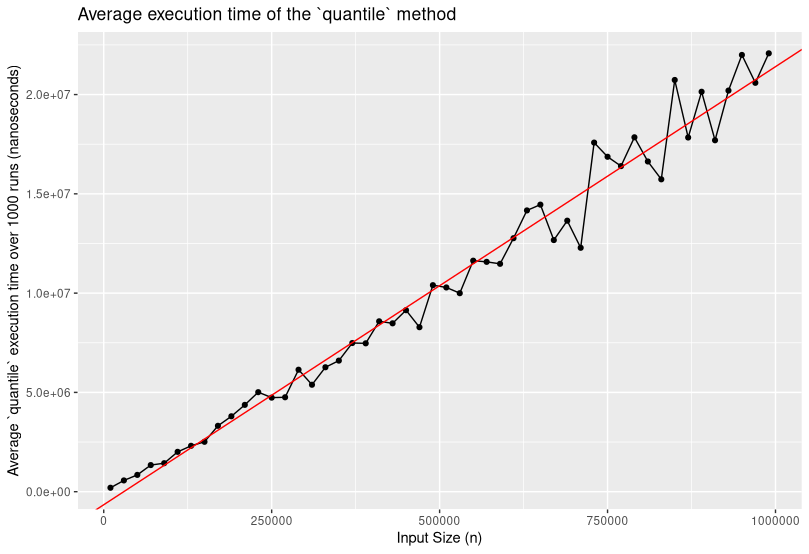
\includegraphics[width=0.7\linewidth]{MonteCarloExecutionTimeTVaR.png}
    \caption{Plot of the execution time of the \texttt{quantile} method}
    \label{fig: quantile execution time}
\end{figure}

\subsection{Closed form method}
As explained in subsection \ref{subsection: generic results}, the closed form expression we found needs a vector $\beta$ of ``seed values'' so that Pearson's correlation $\rho_i := \Corr(Y_i, \Lambda)$ is positive for every $i$. Since we generate a correlation matrix consisting exclusively of positive entries (which implies that the covariances are also positive), a sufficient condition for this to occur, is to take $\beta_i > 0, \forall i$. The covariance between two lognormals with Gaussian copula is known to be $$ \exp \left(\mu_i + \mu_j + \frac{\sigma_i^2 + \sigma_j^2}{2} \right) \cdot (\exp (R_{i j} \sigma_i \sigma_j) - 1) $$ where $R_{i j}$ is the entry in the $i$-th row and the $j$-th column of the correlation matrix $R$. We can calculate the exact correlation between $Y_i$ and $\Lambda$ as follows, making use of the fact that covariance is a bilinear form and that $\Var(X) = \Cov(X, X)$:

\begin{align*}
    &\Corr(Y_i, \Lambda) = \frac{\Cov(Y_i, \sum_j \beta_j Y_j)}{\sqrt{\Var(Y_i) \cdot \Var(\sum_j \beta_j Y_j)}} \\
    &= \frac{\sum_j \beta_j \Cov(Y_i, Y_j)}{\sqrt{\Cov(Y_i, Y_i) \cdot \Cov(\sum_j \beta_j Y_j, \sum_k \beta_k Y_k)}} \\ 
    &= \frac{\sum_j \beta_j \exp \left(\mu_i + \mu_j + \frac{\sigma_i^2 + \sigma_j^2}{2} \right) \cdot (\exp (R_{i j} \sigma_i \sigma_j) - 1)}{\sqrt{\left(\exp \left(2 \mu_i + \sigma_i^2 \right) \cdot (\exp ( \sigma_i^2) - 1)\right) \cdot \left(\sum_j \sum_k \beta_j \beta_k \exp \left(\mu_j + \mu_k + \frac{\sigma_j^2 + \sigma_k^2}{2} \right) \cdot (\exp (R_{j k} \sigma_j \sigma_k) - 1)\right)}}
\end{align*}

This expression is quite unsightly but fortunately we only need to calculate it once per sample. 

%A naturally arising question concerns the selection of \say{good} $\beta$'s. Since we have calculated a lower bound, we want the $\beta$'s to be as variant as possible. We can do this using a fairly crude optimisation algorithm, which is discussed in more detail in the appendix. For the experiments with a high dimension (i.e. the number of individual risks we consider), the $\beta$-optimisation step is skipped, since this is very slow for such cases\footnote{For more information on this optimisation step, see the appendix.}.

A naturally arising question concerns the selection of \say{good} $\beta$'s. By Proposition \ref{prop: inequality of variances convex order} the variance of $S^l$ is always less than the variance of $S$. Thus we want to choose the $\beta$'s such that the variance of $S^l$ captures as much of the variance of $S$ as possible. We can do this using a fairly crude optimisation algorithm, which is discussed in more detail in the appendix. For the experiments with a high dimension (i.e. the number of individual risks we consider), the $\beta$-optimisation step is skipped, since this is very slow for such cases\footnote{For more information on this optimisation step, see the appendix.}.

To illustrate the importance of the choice of $\beta$, let us highlight a small example. Consider the following parameters: $$ R = \begin{bmatrix}
    1.000 & 0.684& 0.998 \\
    0.684 & 1.000 & 0.643 \\
    0.998 & 0.643 & 1.000
\end{bmatrix}, \quad \beta_1 = \begin{bmatrix}5 \\ 1 \\ 1 \end{bmatrix}, \beta_2 = \begin{bmatrix}1 \\ 5 \\ 1 \end{bmatrix}, \beta_3 = \begin{bmatrix}1 \\ 1 \\ 5 \end{bmatrix} $$ 
for a small $n = 3$ simulation. The choice of the $\beta$ vector has a subtle but noticeable influence on the Tail Value-at-Risk predictions. We compare the closed-form TVaR calculations against a fairly large Monte Carlo simulation (sample size $10^5$). Figure \ref{fig: comparing different betas} shows the absolute error for the lower bound estimations for the different $\beta$'s. We see that the results we get from using $\beta_2$ seem less accurate than the estimations resulting from using $\beta_1$ or $\beta_2$. As a result of Proposition \ref{prop: tvar consistent with convex order}, we expect these absolute errors to be greater than zero since $\text{TVaR}_p[S^l] \leq \text{TVaR}_p[S]$ for all $p\in(0,1)$.  In Figure \ref{fig: comparing different betas} we see that this is indeed the case.
\begin{figure}[h!]
    \centering
    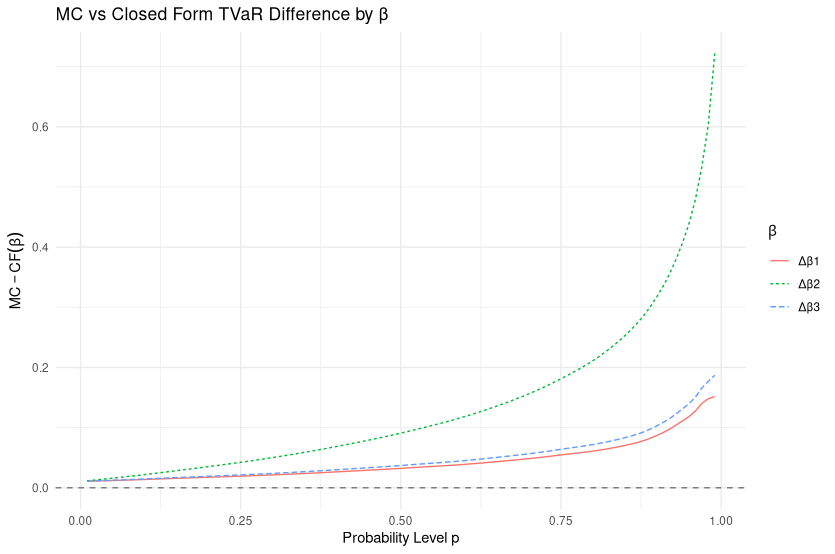
\includegraphics[width=1\linewidth]{AccuracyDifferentBetasTVaR.png}
    \caption{Absolute errors for the different $\beta$ vectors.  \label{fig: comparing different betas}}
\end{figure}

In Table \ref{tab:betaComparison_dif} we compare the covariances with the drawn sample $\lVert \Cov(Y, Y \cdot \beta_i) \rVert_2$ and the sum of the absolute difference with the Monte Carlo value $\sum_p \left|\text{MC}_p - \text{CF}_p(i)\right|$ for the different $\beta$ vectors. We notice that a higher value for the covariance corresponds to a lower error. We could try to explain this by looking at the variance of $S^l$ and trying to maximize this value for different $\beta$'s (and thus different values for the covariance), but these calculations fall outside the scope of this report.


\begin{table}[h!]
	\centering
	\begin{tabular}{ccc}
		$i$ & $\lVert \Cov(Y, Y \cdot \beta_i) \rVert_2$ & $\sum_p \left|\text{MC}_p - \text{CF}_p(i)\right|$ \\
		1 & 1.569771 & 4.179332 \\
		2 & 1.554562 & 13.45786 \\
		3 & 1.557518 & 4.852244 \\
	\end{tabular}
	\caption{$\beta$ comparison error and covariance \label{tab:betaComparison_dif}}
\end{table}
\subsection{Comparison of execution time and accuracy in function of sample size}

The procedures outlined above can be compared on two fronts, both of practical concern: how accurate are the methods, and how quickly can we calculate the results? In both cases, the closed-form for the lower bound is a very satisfactory estimator.

As discussed in Subsection \ref{Subsection: Monte Carlo}, the Monte Carlo computation time scales linearly with the sample size.  A larger sample size improves the accuracy of this estimation, but comes with a proportional computation cost. Throughout this analysis, we work with sample sizes of at least $10^5$, for which we consider the Monte Carlo estimates sufficiently close to the true TVaR of $S$ to serve as a reference value for evaluating the closed-form lower bound. 

The computational cost of the closed-form estimation only depends on the dimension (the number of individual risks we consider). Figure \ref{fig: computation times closed-form} shows the computation times in function of the dimension. Here we used the average of 100 repetitions, the small variations can be attributed to the computer and software. The values of the $\beta$ vector were chosen uniformly in the range $(1,2)$, without optimization\footnote{see the appendix}. We can compare this to the (approximated) computation time for the Monte Carlo calculations as studied in Subsection \ref{Subsection: Monte Carlo}. If we take a sample size of $10^5$ we can use the equation \eqref{eq: computation time MC} \footnote{notice that $n$ in this equation refers to the sample size and not the dimension.} to see that the Monte Carlo method would take about $1550 \; \mu\text{s}$.  So for a fixed dimension of $n = 10$ (and a fixed choice of the $\beta$ vector)  the closed-form calculations are a lot faster than the Monte Carlo estimation.

%The advantage of this trade off is that we can influence the accuracy of this estimation by varying the sample size. In comparison, the closed-form lower bound for the Tail Value-at-Risk only depends on $n$, the amount of individual risks. If this lower bound is not accurate enough, we would have to choose a new vector $\beta$ to improve this estimation. 

One might then rightfully ask if the trade-off is then made in terms of accuracy.  Although Proposition \ref{prop: tvar consistent with convex order} only guarantees a lower bound, Figure \ref{fig:directComparison} seems to indicate that the closed-form approximation approaches the Monte Carlo estimation quite well. This is confirmed by Figure \ref{fig: relative error}: the relative error (with respect to the Monte Carlo estimate) does not exceed $0.1\%$.  The relevant calculated estimations for the Tail Value-at-Risk for $p\in [0.8,1)$ can be found in Figure \ref{fig: estimations in table}. 


The closed-form estimation seems to be more efficient than the Monte Carlo estimation while remaining fairly accurate.  It is important to note, however, that the risks used for those calculations were $X_i \sim \text{Lognormal}(\mu_i,\sigma_i^2)$ with $i\in\{1,2,\dots,10\}$ and $\sigma_i\in (0,0.1)$. The accuracy of the closed form method drastically decreases with increasing standard deviations. Figure \ref{fig: sigmaVgl} shows a comparison of different ranges for the standard deviations, with the x-axes showing the probability level and the y-axes the relative errors (with respect to the Monte Carlo estimates) of the estimates provided by the different methods. We see that the errors are significantly larger if the $\sigma_i$'s are chosen in wider ranges. For example: for $\sigma$'s chosen in in the range $[0.01,5]$ we see that the relative error exceeds $20\%$ for $p \geq 0.75$.

\begin{figure}[h!]
	\centering
	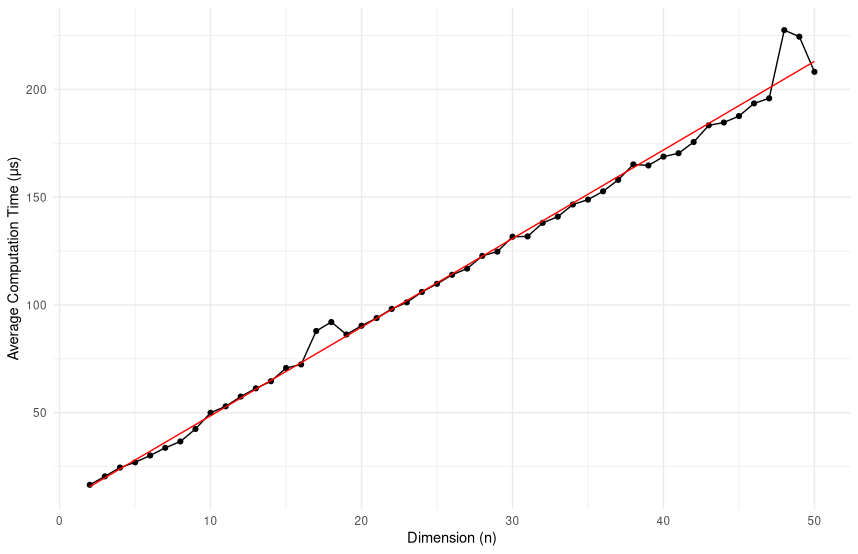
\includegraphics[width=1\linewidth]{ComputationTimesClosedForm.png}
	\caption{Computation times closed-form estimation.  \label{fig: computation times closed-form}}
\end{figure}
\begin{figure}[h!]
	\centering
	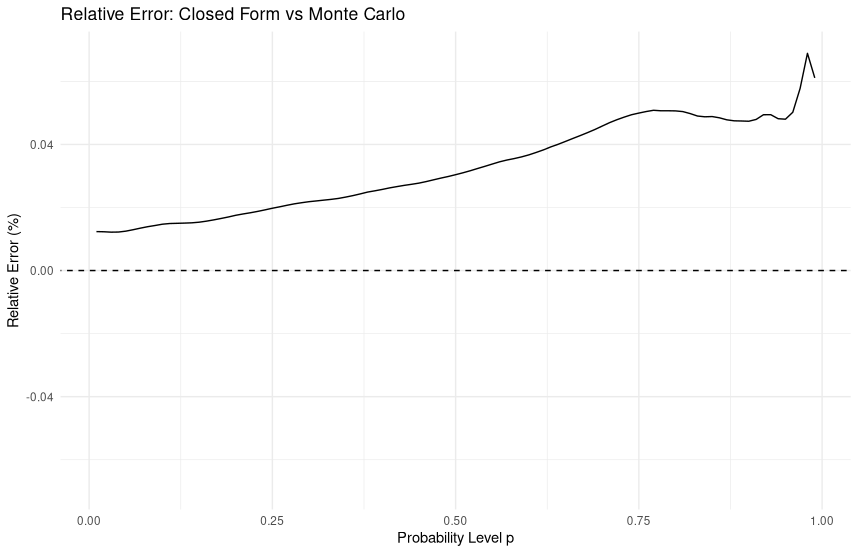
\includegraphics[width=1\linewidth]{RelativeErrorTVaR.png}
	\caption{Relative error closed-form estimation.  \label{fig: relative error}}
\end{figure}
\begin{figure}[h!]
	\centering
	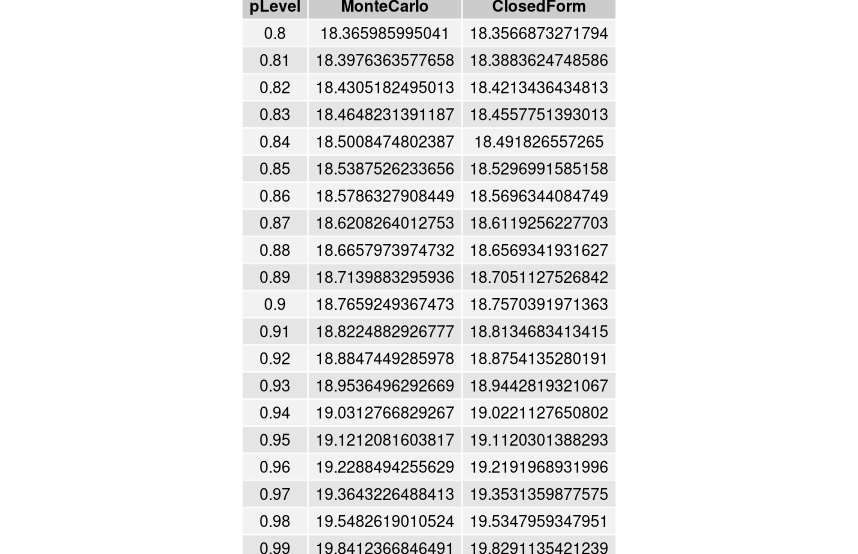
\includegraphics[width=1\linewidth]{TabelTVaREstimates.png}
	\caption{Estimations for $\text{TVaR}_p[S]$ with $p\in [0.8,1)$.  \label{fig: estimations in table}}
\end{figure}
\begin{figure}[h!]
	\centering
	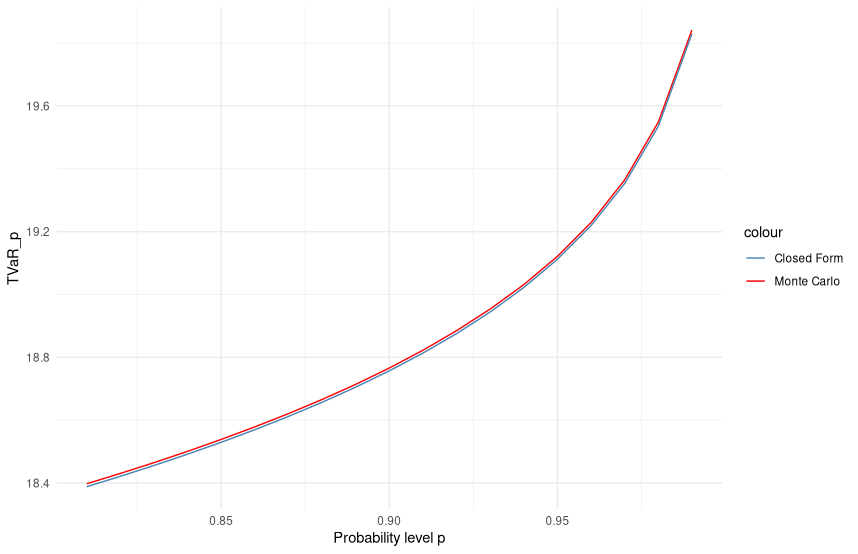
\includegraphics[width=0.9\linewidth]{DirectComparisonTVaR.png}
	\caption{$\text{TVaR}_p$ predictions for $p\in (0.8,1)$ with $n = 10$, sample size = 5e5 \label{fig:directComparison}}
\end{figure}
\begin{figure}[h!]
    \centering
    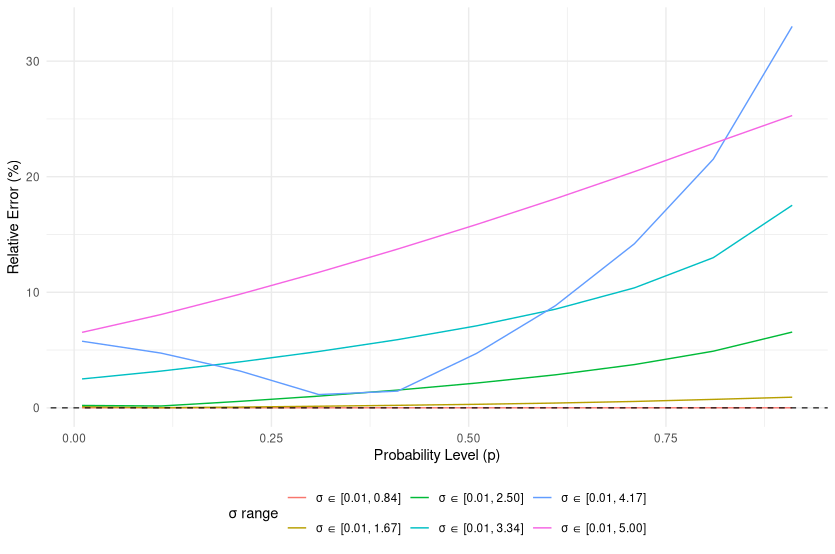
\includegraphics[width=1\linewidth]{DifferentSigmasTVaR.png}
    \caption{Relative error of the lower bound estimate for different ranges of $\sigma$ \label{fig: sigmaVgl}}
\end{figure}

\subsection{Conclusion}
In this section we have combined the theory of the previous sections to get a general idea of the behaviour of the lower bound $S^l$ for $S$. We started from lognormal distributed risks $X_i$ for $i\in \{1,2,\dots,n\}$ with a Gaussian copula. We compared two methods to estimate the Tail Value-at-Risk of $S = \sum_{i=1}^n X_i$: the Monte Carlo estimation and the closed-form of the lower bound $S^l$ as calculated in Subsection \ref{subsection: generic results} in Section \ref{section: upper and lower bounds}. 

For large sample sizes we may assume that the Monte Carlo estimation is an accurate approximation of the true value of the TVaR, but this comes with expensive computational costs since the computation time increases linearly with the sample size. The calculations of the closed-form expressions of the lower bound of the TVaR are a lot cheaper in computation time, these only depend on the amount of individual risks $n$. 

While the TVaR of $S^l$ is merely a lower bound of the TVaR of $S$, it turns out that these estimations can be quite accurate, depending on the distribution parameters of the $X_i$'s and the choice of the $\beta$ vector.
%Standard error deviation (Cox and Hinkley, 1974 estimator)

\section{Conclusion}

In this report, we explored some foundational concepts from quantitative risk measurement. We introduced some common examples of risk measures and copulas, explored stochastic orderings and their application on these risk measures. An upper bound, but more pertinently a lower bound, on the Value-at-Risk and Tail Value-at-Risk, and found a closed form expression for these bounds. Finally, this closed form expression was implemented in \texttt{R}, and the calculation speed and accuracy were compared to a routine Monte Carlo implementation. If the variances of the lognormals are small enough, the closed form for the lower bound forms an especially satisfactory estimation.

\printbibliography

\newpage
\section*{Appendix A: a discussion of the optimisation algorithm}
Finding an optimal $\beta$ is done via quite a crude optimisation algorithm, whereby we define an initial search space for the $\beta$'s as an interval $[\beta_\text{min}, \beta_\text{max}]^{\otimes n}$, divide this up along each axis into a fixed number $k$ of equally spaced points to get $k^n$ evaluation points, evaluate the correlation in each of those grid points and store the one with the highest Euclidean norm. We use the built-in \texttt{cor} routine for this to make the code a bit more sightly: in practice the empirical correlation and the theoretical one are close enough. We then define a new search space around this highest value and refine the search; this is done recursively and stops once a desired precision has been reached.

\begin{lstlisting}[language=R, caption=Beta optimisation routine]
findBestβ <- function(minV, maxV, sieve, iterationsLeft) {
  stepSizes <- (maxV - minV) / sieve
  linspaces <- lapply(1:n, function(i) seq(from = minV[i], to = maxV[i], by = stepSizes[i]))
  searchSpace <- expand.grid(linspaces, KEEP.OUT.ATTRS = FALSE)
  
  bestβ = rep(NA, n)
  bestCor = -Inf
  
  for (i in 1:sieve^n) {
    β <- c(searchSpace[i, 1:n], use.names = FALSE, recursive = TRUE)
    correlation <- cor(Y, Y %*% β)
    euclNorm <- (t(correlation) %*% correlation)[1,1]
    if (euclNorm > bestCor) {
      bestβ <- β
      bestCor = euclNorm
    }
  }
  
  message(sprintf("best β with %d iterations left is %s", iterationsLeft, paste(bestβ, collapse = ", ")))
  
  if (iterationsLeft == 0) {
    return(bestβ)
  } else {
    return(findBestβ(bestβ - stepSizes / 2, bestβ + stepSizes / 2, sieve, iterationsLeft - 1))
  }
}
\end{lstlisting}

One can rightfully remark that such a procedure will only produce the optimal value for $\beta$ if the function $\beta \mapsto \Corr(Y_i, \sum_i \beta_i Y_i)$ tends to a global maximum, and if this global maximum lies within our initial search space. While this is true, a visual analysis of the effects of varying different coordinates of $\beta$ seems to indicate that this is indeed the case:

\begin{figure}
    \centering
    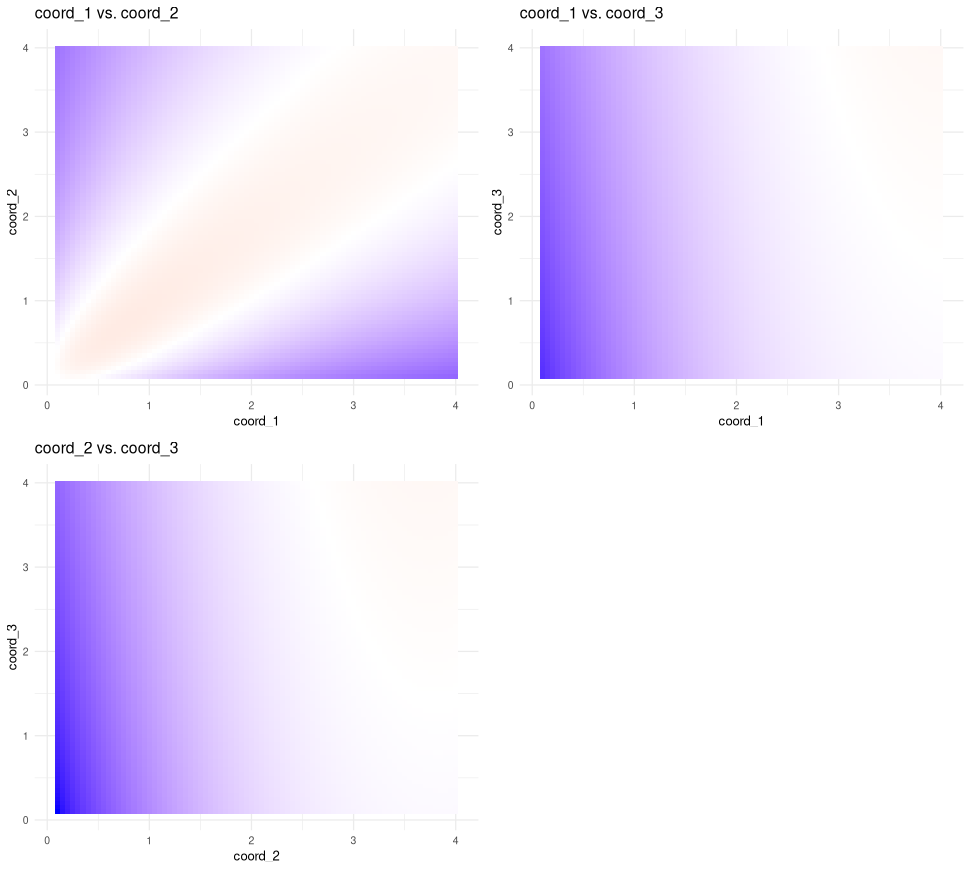
\includegraphics[width=1\linewidth]{Correlations.png}
    \caption{The correlations between different coordinates}
\end{figure}

\newpage

\section*{Appendix B: code}

\begin{lstlisting}[language=R]
library(mvtnorm)
library(ggplot2)
library(ggExtra)
library(sn)
library(twopiece)
library(plotly)
library(copula)
library(PerformanceAnalytics)
library(tidyr)
library(dplyr)

## Different copulas with lognormal marginal distributions

n  <- 50000
m <- 2

# Frank's copula
alpha <- 55
frankCop <- frankCopula(alpha, m)
U1 <- rCopula(n, frankCop)
X1 <- qnorm(U1, mean = 0, sd = 1)
df1 <- as.data.frame(X1)
colnames(df1) <- c("x","y")

# Gaussian copula
correlation <- cor(U1)
rho <- correlation[1,2]

gaussianCop <- normalCopula(rho, m, dispstr = "ex")
U2 <- rCopula(n, gaussianCop)
X2 <- qnorm(U2, mean = 0, sd = 1)
df2 <- as.data.frame(X2)
colnames(df2) <- c("x","y")

df1$Copula <- "Frank's"
df2$Copula <- "Gaussian"
df <- rbind(df1, df2)
df <- df[sample(nrow(df)), ] # shuffle the rows to avoid any ordering effects in the plot

ggplot(df, aes(x, y, color = Copula)) + 
  geom_point(size = .5) + 
  theme(axis.text.x = element_text(size = 14), axis.text.y = element_text(size = 14)) +
  xlab("X") + ylab("Y") +
  scale_color_manual(values = c("darkred", "steelblue")) +
  labs(color = "Copula type") +
  theme(legend.title = element_text(size = 14), legend.text = element_text(size = 12))

## Aggregate loss with different copulas 

n  <- 10000
m <- 100

rho <- 0.7

gaussianCop <- normalCopula(rho, m, dispstr = "ex")
U <- rCopula(n, gaussianCop)

X <- qlnorm(U, meanlog = 0, sdlog = 1)
S <- rowSums(X)

var <- quantile(S, 0.99)
tvar <- mean(S[S > var])

ggplot(data.frame(S), aes(S)) +
  geom_histogram(bins = 60, fill = "darkred", color = "white") +
  geom_vline(aes(xintercept = var, color = "VaR 0.99"), linewidth = 0.5) +
  geom_vline(aes(xintercept = tvar, color = "TVaR 0.99"), linewidth = 0.5) +
  scale_color_manual(values = c("VaR 0.99" = "steelblue", "TVaR 0.99" = "palevioletred")) +
  labs(x = "Total Loss S", y = "Frequency", color = "Risk Measure") + 
  theme(legend.position = c(1, 1), legend.justification = c(1, 1))

## Value-at-risk and Tail value-at-risk

n  <- 25000
m <- 10
repetitions <- 50

rho <- seq(0, 0.99, 0.05)
results <- data.frame()

for (r in 1:length(rho)){
  for (repetition in 1:repetitions) {
    gaussianCop <- normalCopula(rho[r], m, dispstr = "ex")
    U <- rCopula(n, gaussianCop)
    X <- qlnorm(U, meanlog = 0, sdlog = 1)
    S <- rowSums(X)
    
    var <- quantile(S, 0.99)
    tvar <- mean(S[S > var])
    
    results <- rbind(results, data.frame(rho = rho[r], repetition = repetition, VaR = var, TVaR = tvar))
  }
}

summary_df <- results %>%
  group_by(rho) %>%
  summarise(min_VaR = min(VaR), max_VaR = max(VaR), mean_VaR = mean(VaR),
            min_TVaR = min(TVaR), max_TVaR = max(TVaR), mean_TVaR = mean(TVaR))

p1 <- ggplot() +
  geom_line(data=results, aes(x=rho, y=VaR, group=repetition), alpha=0.3, color="gray") +
  geom_ribbon(data=summary_df, aes(x=rho, ymin=min_VaR, ymax=max_VaR), alpha=0.3, fill="lightblue") +
  geom_line(data=summary_df, aes(x=rho, y=mean_VaR), color="black", linewidth=1.5) +
  labs(
    x = expression(Correlation),
    y = "Value-at-Risk (q = 0.99)"
  ) +
  theme_minimal(base_size = 16)
p1

p2 <- ggplot() +
  geom_line(data=results, aes(x=rho, y=TVaR, group=repetition), alpha=0.3, color="gray") +
  geom_ribbon(data=summary_df, aes(x=rho, ymin=min_TVaR, ymax=max_TVaR), alpha=0.3, fill="lightcoral") +
  geom_line(data=summary_df, aes(x=rho, y=mean_TVaR), color="black", linewidth=1.5) +
  labs(
    x = expression(Correlation),
    y = "Tail Value-at-Risk (q = 0.99)"
  ) +
  theme_minimal(base_size = 16)
p2
\end{lstlisting}

\begin{lstlisting}[language=R]
library(ggplot2)
library(copula)
library(microbenchmark)
library(gridExtra)
library(tidyr)
library(dplyr)
library(patchwork)
library(broman)
library(kableExtra)


generateCorrelationMatrix <- function(n) {
  # We first generate a correlation matrix:
  Loadings <- matrix(runif(n^2, 0, 1), nrow = n)
  Symm <- Loadings %*% t(Loadings)
  D <- diag(1 / sqrt(diag(Symm)))
  
  D %*% Symm %*% D
}

runAll <- function(
    trials, 
    n, 
    correlationMatrix = NULL,
    βGiven = NULL,
    μRange = list(min = -1, max = 1),
    σRange = list(min = 0, max = 1),
    μGiven = NULL,
    σGiven = NULL,
    pValues = seq(0, 0.99, by = 0.01), 
    microbenchmarkControl = list(warmup = 20, replications = 50), 
    optimiseBeta = FALSE,
    inspectCorrelation = NULL) {
  message(sprintf("Running with %d trials and %d dimensions", trials, n))
  
  if (is.null(correlationMatrix)) {
    R <- generateCorrelationMatrix(n)
  } else {
    R <- correlationMatrix
  }
  
  gaussianCopula <- normalCopula(param = R[lower.tri(R)],
                                 dim = n,
                                 dispstr = "un")
  Unif <- rCopula(trials, gaussianCopula)
  
  # Get some interesting parameters for the lognormal distributions
  if (is.null(μGiven)) {
    μ = runif(n, min = μRange$min, max = μRange$max)
  } else {
    μ = μGiven
  }
  
  if (is.null(σGiven)) {
    σ = runif(n, min = σRange$min, max = σRange$max)
  } else {
    σ = σGiven
  }
  
  multivariateDist <- mvdc(
    copula = gaussianCopula,
    margins = rep("lnorm", n),
    paramMargins = lapply(1:n, function(i) list(meanlog = μ[i], sdlog = σ[i]))
  )
  
  samplingTime <- summary(microbenchmark(
    rMvdc(trials, multivariateDist), 
    unit = "us", 
    control = microbenchmarkControl
  ))
  
  Y <- rMvdc(trials, multivariateDist)
  S <- rowSums(Y)
  
  df <- data.frame()
  
  # Find some vector β such that Cor(Y, β · Y) is high; for simplicity we will do
  # this using the builtin cor() function since that simplifies the code a bit
  
  findBestβ <- function(minV, maxV, sieve, iterationsLeft) {
    stepSizes <- (maxV - minV) / sieve
    linspaces <- lapply(1:n, function(i) seq(from = minV[i], to = maxV[i], by = stepSizes[i]))
    searchSpace <- expand.grid(linspaces, KEEP.OUT.ATTRS = FALSE)
    
    bestβ = rep(NA, n)
    bestCor = -Inf
    
    for (i in 1:sieve^n) {
      β <- c(searchSpace[i, 1:n], use.names = FALSE, recursive = TRUE)
      correlation <- cor(Y, Y %*% β)
      euclNorm <- (t(correlation) %*% correlation)[1,1]
      if (euclNorm > bestCor) {
        bestβ <- β
        bestCor = euclNorm
      }
    }
    
    message(sprintf("best β with %d iterations left is %s", iterationsLeft, paste(bestβ, collapse = ", ")))
    
    if (iterationsLeft == 0) {
      return(bestβ)
    } else {
      return(findBestβ(bestβ - stepSizes / 2, bestβ + stepSizes / 2, sieve, iterationsLeft - 1))
    }
  }
  
  # since we chose the correlation matrix to be positive definite, any choice of
  # β's with ∀ i: βᵢ > 0 will lead to a positive correlation between Y and Λ.
  if (is.null(βGiven)) {
    if (optimiseBeta) {
      β <- findBestβ(rep(1, n), rep(5, n), 3, 5)
    } else {
      β <- runif(n, min = 1, max = 2)
    }
  } else {
    β <- βGiven
  }
  
  # The following is debug code to draw a heatmap for correlations associated with β's 
  # to check if there is some global maximum to aim for
  # if this is not the case, the whole endeavour is futile
  # because of the huge expand.grid, we will only do this for a small number of 
  # coordinates and a coarse grid, but it should be enough to get an idea of the landscape
  if (!is.null(inspectCorrelation)) {
    linspace <- seq(from = inspectCorrelation$from, to = inspectCorrelation$to, by = inspectCorrelation$by)
    searchSpace <- expand.grid(lapply(1:n, function(x) linspace))
    
    gridDF <- data.frame()
    
    progress <- txtProgressBar(max=(length(linspace)^n), initial=0, style=3, char="#")
    
    for (i in 1:(length(linspace)^n)) {
      β <- c(searchSpace[i, 1:n], use.names = FALSE, recursive = TRUE)
      # message(paste(β, collapse = ", "))
      correlation <- cor(Y, Y %*% β)
      euclNorm <- (t(correlation) %*% correlation)[1,1]
      
      coordValues <- as.list(β)
      names(coordValues) <- lapply(1:n, function (num) paste("coord_", num, sep=""))
      
      value <- c(val = euclNorm, coordValues)
      
      # store the position and value for the heatmap
      gridDF <- rbind(gridDF, value)
      
      setTxtProgressBar(progress, i)
    }
    
    # view pairwise plots as heatmaps per coordinate pair in a grid
    plotList <- list()
    for (i in 1:(n-1)) {
      for (j in (i+1):n) {
        plotList[[length(plotList) + 1]] <- ggplot(gridDF, aes_string(x = paste("coord_", i, sep=""), y = paste("coord_", j, sep=""))) +
          geom_tile(aes(fill = val)) +
          scale_fill_gradient2(low = "blue", mid = "white", high = "red", midpoint = quantile(gridDF[,"val"], 0.75)) +
          labs(title = sprintf("coord_%d vs. coord_%d", i, j), x = sprintf("coord_%d", i), y = sprintf("coord_%d", j)) +
          theme_minimal() + 
          guides(fill="none")
      }
    }
    
    
    do.call("grid.arrange", c(plotList, ncol = n-1))
    return(gridDF)
  }
  
  
  {
    # theoretical covariance between Yᵢ and Yⱼ:
    tCov <- function(i, j) {
      exp(μ[i] + μ[j] + 0.5 * (σ[i]^2 + σ[j]^2)) * (exp(R[i, j] * σ[i] * σ[j]) - 1)
    }
    
    # Theoretical correlation between Y and Λ, making use of the fact that Cov is a bilinear form:
    VarΛ = sum(sapply(1:n, function(i) {
      sum(sapply(1:n, function(j) { β[i] * β[j] * tCov(i, j) }))
    }))
    
    ρ = sapply(1:n, function(i) {
      nom = sum(sapply(1:n, function(j) { β[j] * tCov(i, j) }))
      den = sqrt(tCov(i, i) * VarΛ)
      nom / den
    })
    
    rm(tCov, VarΛ)
  }
  
  if (length(pValues) == 1) {
    progress <- txtProgressBar(
      min = 0,
      max = max(pValues),
      initial = 0,
      style = 3,
      char = "#")
  } else {
    progress <- txtProgressBar(
      min = min(pValues), 
      max = max(pValues), 
      initial = min(pValues), 
      style = 3, 
      char = "#")
  }
  
  for (p in pValues) {
    mc2 = microbenchmark(mean(S[S > quantile(S, p)]), unit = "us", control = microbenchmarkControl)
    cf2 = microbenchmark(sum(sapply(1:n, function(i) {
          b = μ[i] + 0.5 * (1 - ρ[i]^2) * σ[i]^2
          exp(b + (σ[i]^2 * ρ[i]^2) / 2) * pnorm(σ[i]* ρ[i] - qnorm(p))
          }))  / (1-p), unit = "us", control = microbenchmarkControl)
    
    TVaR_monteCarlo = mean(S[S > VaR_monteCarlo])
    TVaR_closedForm = sum(sapply(1:n, function (i) {
      b = μ[i] + 0.5 * (1 - ρ[i]^2) * σ[i]^2
      exp(b + (σ[i]^2 * ρ[i]^2) / 2) * pnorm(σ[i]* ρ[i] - qnorm(p))
    }))  / (1-p)
    
    df <- rbind(df, list(
      pLevel = p, 
      MC2 = TVaR_monteCarlo,
      CF2 = TVaR_closedForm,
      
      MC2TimeAvg = summary(mc2)$mean + samplingTime$mean,
      CF2TimeAvg = summary(cf2)$mean,
      MCTimeMax = summary(mc)$max + samplingTime$max,
      CFTimeMax = summary(cf)$max,
      MC2TimeMax = summary(mc2)$max + samplingTime$max,
      CF2TimeMax = summary(cf2)$max,
      
      MCError = quantileEstimation[[2]]
    ))
    
    setTxtProgressBar(progress, p)
  }
  
  message(sprintf("avg Monte Carlo time: %f μs, avg closed form time: %f μs", mean(df$MCTimeAvg), mean(df$CFTimeAvg)))
  
  rm(list = ls() %>% setdiff(c("df")))
  
  df
}

execution_times <- data.frame()
avgRuns <- 2
for (trials in seq(10e4, 50e4, by = 10e4)) {
  mcTimes <- numeric(avgRuns)
  cfTimes <- numeric(avgRuns)
  mc2Times <- numeric(avgRuns)
  cf2Times <- numeric(avgRuns)
  
  for (i in 1:avgRuns) {
    result <- runAll(trials = trials, n = 10, pValues = seq(0.1, 0.9, by = 0.1))
    mcTimes[i] <- mean(result$MCTimeAvg)
    cfTimes[i] <- mean(result$CFTimeAvg)
    mc2Times[i] <- mean(result$MC2TimeAvg)
    cf2Times[i] <- mean(result$CF2TimeAvg)
  }
  
  execution_times <- rbind(execution_times, list(
    trials = trials, 
    MCTimeMin = min(mcTimes),
    MCTimeAvg = mean(mcTimes),
    MCTimeMax = max(mcTimes),
    CFTimeMin = min(cfTimes),
    CFTimeAvg = mean(cfTimes),
    CFTimeMax = max(cfTimes),
    MC2TimeMin = min(mc2Times),
    MC2TimeAvg = mean(mc2Times),
    MC2TimeMax = max(mc2Times),
    CF2TimeMin = min(cf2Times),
    CF2TimeAvg = mean(cf2Times),
    CF2TimeMax = max(cf2Times)
  ))
}


speedup <- mutate(execution_times, Speedup = MC2TimeAvg / CF2TimeAvg)

ggplot(speedup, aes(x = trials)) +
  geom_line(aes(y = Speedup), color = "blue") +
  labs(title = "Speedup of Closed Form over Monte Carlo", x = "Number of trials", y = "Speedup (Closed Form Time / Monte Carlo Time)") +
  theme_minimal()

# split the plot into two subplots to better visualize the time ranges
pivoted <- execution_times %>%
  select(trials, starts_with("MC2"), starts_with("CF2")) %>%
  pivot_longer(
    cols = -trials,
    names_to = c("Method", ".value"),
    names_pattern = "(MC2|CF2)Time(Min|Avg|Max)"
  )

pivoted$Method <- recode(pivoted$Method,
                         MC2 = "Monte Carlo",
                         CF2 = "Closed Form")

ggplot(pivoted, aes(x = trials)) +
  geom_line(aes(y = Avg, colour = Method)) +
  geom_ribbon(aes(ymin = Min, ymax = Max, fill = Method), alpha = 0.2) +
  labs(title = "Average computation time for Closed form vs. Monte Carlo (sample size 1e6)", x = "Number of trials", y = "Average Time (μs)") +
  theme_minimal() +
  theme(legend.position = "none") + 
  facet_wrap(~Method, scales = "free_y")



# We can also look at individual calculation times in more detail

df <- runAll(
  trials = 100000, 
  n = 10, 
  pValues = seq(0.01, 0.99, by = 0.01), 
  σRange = list(min = 0, max = 0.1),
  microbenchmarkControl = list(warmup = 0, replications = 0),
  optimiseBeta = FALSE)

ggplot(subset(df, pLevel > 0.8), aes(x = pLevel)) +
  geom_line(aes(y = MC2, color = "Monte Carlo")) +
  geom_line(aes(y = CF2, color = "Closed Form")) +
  
  labs(x = "Probability level p", y = "TVaR_p") +
  scale_color_manual(values = c("steelblue", "red", "red", "red")) +
  theme(legend.title = element_blank()) + 
  theme_minimal()

stErrDeviation <- df %>%
  select(MC2, CF2, MCError, pLevel) %>%
  filter(MCError != 0) %>%
  mutate(StdErrDev = (CF2 - MC2) / MCError)

maxDev = max(abs(stErrDeviation$StdErrDev))

ggplot(data = stErrDeviation, aes(x = pLevel)) +
  geom_line(aes(y = StdErrDev)) + 
  geom_abline(intercept = 1, slope = 0, linetype = "dashed") + 
  geom_abline(intercept = -1, slope = 0, linetype = "dashed") +
  ylim(-maxDev, maxDev) + 
  geom_ribbon(aes(ymin=1, ymax=maxDev), fill="red", alpha=0.2) + 
  geom_ribbon(aes(ymin=-maxDev, ymax=-1), fill="red", alpha=0.2)


relativeError <- df %>%
  select(MC2, CF2, pLevel) %>%
  mutate(RelErr = ( MC2 - CF2) / MC2 * 100)  

maxRelErr = max(abs(relativeError$RelErr))

ggplot(data = relativeError, aes(x = pLevel)) +
  geom_line(aes(y = RelErr)) +
  geom_abline(intercept = 0, slope = 0, linetype = "dashed") +
  ylim(-maxRelErr, maxRelErr) +
  labs(
    title = "Relative Error: Closed Form vs Monte Carlo",
    x = "Probability Level p",
    y = "Relative Error (%)"
  ) +
  theme_minimal()

deelDf <- subset(df, pLevel >= 0.8)
deelDf <- deelDf %>% select(pLevel, MC2, CF2)
deelDf <- deelDf %>% rename(MonteCarlo = MC2, ClosedForm = CF2)

grid.table(deelDf, rows = NULL)
  

differences <- df %>%
  mutate(Difference = MC2 - CF2) %>%
  mutate(DifferenceWhenCFExceeds = ifelse(Difference < 0, Difference, NA))

differences <- subset(differences, pLevel != 0)

ggplot(differences, aes(x = pLevel)) +
  geom_abline(intercept = 0, slope = 0, linetype = "dashed", color = "black") +
  geom_area(aes(y = DifferenceWhenCFExceeds), fill = "red", alpha = 0.2) + 
  geom_line(aes(y = Difference), color = "blue") +
  labs(title = "Difference between Closed Form and Monte Carlo VaR estimates", x = "Probability level p", y = "Difference (Closed Form - Monte Carlo)")

ggplot(subset(df, MCTimeMax < 10000), aes(x = pLevel)) +
  geom_ribbon(aes(ymin = MCTimeMin, ymax = MCTimeMax, fill = "Monte Carlo"), alpha = 0.2) +
  geom_ribbon(aes(ymin = CFTimeMin, ymax = CFTimeMax, fill = "Closed form"), alpha = 0.2) +
  geom_line(aes(y = MC2TimeAvg, colour = "Monte Carlo"), linewidth = 1) +
  geom_line(aes(y = CF2TimeAvg, colour = "Closed form"), linewidth = 1) +
  labs(title = "Computation time for Monte Carlo vs. Closed form (sample size 1e4)", x = "Probability level p", y = "Time (μs)") +
  guides(fill = guide_legend(title = "Method"))


merged_times <- df %>%
  select(pLevel, MC2TimeAvg, CF2TimeAvg) %>%
  pivot_longer(cols = c(MC2TimeAvg, CF2TimeAvg), names_to = "Method", values_to = "Time")

ggplot(subset(merged_times, Time < 400), aes(x = Time, fill=Method)) +
  geom_histogram(binwidth=4, alpha=0.9, position="identity") +
  theme_minimal()

# inspect correlation
gridDF <- runAll(
  trials = 50, 
  n = 3, 
  pValues = seq(0, 0.99, by = 0.01), 
  microbenchmarkControl = list(warmup = 20, replications = 100),
  inspectCorrelation = list(from = 0.5, to = 10, by = 0.15)
)

# by running a very large Monte Carlo simulation, we can get a very good
# estimate of the true VaR for a given set of parameters, and then we can
# compare the closed form estimate to that to see how well it performs for 
# different ranges of σ
σRangePlots <- list()
n = 10
μValues = runif(n, min = -2, max = 2)
pValues = seq(0.01, 0.99, by = 0.1)

rows = 2
cols = 3
σMin = 0.01
σMax = 5
diff = (σMax - σMin) / (rows * cols)

for (σRangeMax in seq(σMin, σMax - diff, by = diff)) {
  message(sprintf("Running for σ range max = %f", σRangeMax))
  σValues = runif(n, min = σRangeMax, max = σRangeMax + diff)
  
  accurateMCResult <- runAll(
    trials = 1e5, 
    n = n, 
    pValues = pValues, 
    microbenchmarkControl = list(warmup = 0, replications = 0),
    μGiven = μValues,
    σGiven = σValues
  )
  
  accurateMCResult <- select(accurateMCResult, pLevel, MC2)
  
  CFResult <- runAll(
    trials = 1e4,
    n = n,
    pValues = pValues,
    microbenchmarkControl = list(warmup = 0, replications = 0),
    μGiven = μValues,
    σGiven = σValues
  )
  
  CFResult <- select(CFResult, pLevel, CF2)
  
  comparison <- merge(accurateMCResult, CFResult, by = "pLevel") %>%
    mutate(σRangeMax = σRangeMax)
  
  plot <- ggplot(data = comparison, aes(x = pLevel)) + 
    geom_line(aes(y = MC2, color = "Monte Carlo"), linewidth = 1) +
    geom_line(aes(y = CF2, color = "Closed form"), linewidth = 1) + 
    labs(title = sprintf("σ ∈ [%.2f, %.2f]", σRangeMax, σRangeMax + diff), y = NULL, x = NULL)
  
  σRangePlots[[length(σRangePlots) + 1]] <- plot
}
wrap_plots(σRangePlots, ncol = 4, guides = "collect") + 
  plot_annotation(title = "Comparison of Monte Carlo and Closed Form VaR estimates for different σ ranges") &
  theme(legend.position = "bottom", legend.title = element_blank())


allResults <- data.frame()

for (σRangeMax in seq(σMin, σMax - diff, by = diff)) {
  message(sprintf("Running for σ range max = %f", σRangeMax))
  σValues = runif(n, min = σMin, max = σRangeMax + diff)
  
  accurateMCResult <- runAll(
    trials = 1e5, 
    n = n, 
    pValues = pValues, 
    σRange = list(min = σMin, max = σRangeMax),
    microbenchmarkControl = list(warmup = 0, replications = 0),
    μGiven = μValues
  ) %>% select(pLevel, MC2, CF2)
  
  comparison <- accurateMCResult %>%
    mutate(
      σRange = sprintf("σ ∈ [%.2f, %.2f]", σMin, σRangeMax + diff),
      RelErr = (MC2 - CF2) / MC2 * 100
    )
  
  allResults <- rbind(allResults, comparison)
}



ggplot(allResults, aes(x = pLevel, y = abs(RelErr), color = σRange)) +
  geom_line(linewidth = 0.5) +
  geom_abline(intercept = 0, slope = 0, linetype = "dashed", alpha = 0.8) +
  labs(
    x = "Probability Level (p)",
    y = "Relative Error (%)",
    color = "σ range"
  ) +
  theme_minimal() +
  theme(legend.position = "bottom")



## Let's inspect the way β's affect the predictions

βComparisonDf <- data.frame()

R <- generateCorrelationMatrix(3)

μ = runif(3, min = -1, max = 1)
σ = runif(3, min =  0, max = 1)

pValues <- seq(0.01, 0.99, by = 0.01)
betas <- tibble(names= c("β1", "β2", "β3"), comp1 = c(5, 1, 1), comp2 = c(1, 5, 1), comp3 = c(1, 1, 5))

gaussianCopula <- normalCopula(param = R[lower.tri(R)], dim = 3, dispstr = "un")

multivariateDist <- mvdc(
  copula = gaussianCopula,
  margins = rep("lnorm", 3),
  paramMargins = lapply(1:3, function(i) list(meanlog = μ[i], sdlog = σ[i]))
)

Y <- rMvdc(100, multivariateDist)

for (i in 1:3) {
  β = c(betas$comp1[i], betas$comp2[i], betas$comp3[i])
  
  {
    # theoretical covariance between Yᵢ and Yⱼ:
    tCov <- function(i, j) {
      exp(μ[i] + μ[j] + 0.5 * (σ[i]^2 + σ[j]^2)) * (exp(R[i, j] * σ[i] * σ[j]) - 1)
    }
    
    # Theoretical correlation between Y and Λ, making use of the fact that Cov is a bilinear form:
    VarΛ = sum(sapply(1:3, function(i) {
      sum(sapply(1:3, function(j) { β[i] * β[j] * tCov(i, j) }))
    }))
    
    ρ = sapply(1:3, function(i) {
      nom = sum(sapply(1:3, function(j) { β[j] * tCov(i, j) }))
      den = sqrt(tCov(i, i) * VarΛ)
      nom / den
    })
    
    rm(tCov, VarΛ)
  }
  
  # covariance size
  euclNorm <- sqrt(sum(ρ^2))
  message(sprintf("beta %s : cov %f", betas$names[i], euclNorm))
  result <- data.frame()
  for (p in pValues) {
    TVaR_closedForm = sum(sapply(1:3, function (i) {
      b = μ[i] + 0.5 * (1 - ρ[i]^2) * σ[i]^2
      exp(b + (σ[i]^2 * ρ[i]^2) / 2)* pnorm(σ[i]* ρ[i] - qnorm(p))
    })) / (1-p)
    
    result <- rbind(result, list(
      pLevel = p, 
      CF2 = TVaR_closedForm,
      βName = betas$names[i]
    ))
    
  }
  
  βComparisonDf <- rbind(βComparisonDf, result)
}

MCValues <- runAll(
  trials = 1e5, 
  n = 3, 
  pValues = pValues, 
  microbenchmarkControl = list(warmup = 0, replications = 0),
  μGiven = μ,
  σGiven = σ,
  βGiven = β,
  correlationMatrix = R
) %>% select(pLevel, MC2)

βComparisonDfMerged <- βComparisonDf %>%
  pivot_wider(names_from = βName, values_from = c(CF2)) %>%
  merge(MCValues, by = "pLevel") %>%
  mutate(Δβ1 = (MC2 - β1)/MC2 * 100, Δβ2 = (MC2 - β2)/MC2 * 100, Δβ3 = (MC2 - β3)/MC2 *100) %>%
  select(pLevel, MC2, Δβ1, Δβ2, Δβ3)


βComparisonDfMerged %>%
  pivot_longer(
    cols = c(Δβ1, Δβ2, Δβ3),
    names_to = "Beta",
    values_to = "Difference"
  ) %>%
  ggplot(aes(x = pLevel, y = Difference, color = Beta, linetype = Beta)) +
  geom_line() +
  geom_hline(yintercept = 0, linetype = "dashed", color = "black", alpha = 0.5) +
  labs(
    title = "MC vs Closed Form TVaR Difference by β",
    x = "Probability Level p",
    y = "Relarive error (%)",
    color = expression(beta),
    linetype = expression(beta)
  ) +
  theme_minimal()

βComparisonDfMerged %>%
  summarise(
    β1 = sum(abs(Δβ1)),
    β2 = sum(abs(Δβ2)),
    β3 = sum(abs(Δβ3))
  )


# computation cost lower bound different dimensions. 

runAll2 <- function(
    n, 
    correlationMatrix = NULL,
    βGiven = NULL,
    μRange = list(min = -1, max = 1),
    σRange = list(min = 0, max = 1),
    μGiven = NULL,
    σGiven = NULL,
    pValues = seq(0, 0.99, by = 0.01), 
    microbenchmarkControl = list(warmup = 20, replications = 50)) {
  message(sprintf("Running with %d dimensions", n))
  
  if (is.null(correlationMatrix)) {
    R <- generateCorrelationMatrix(n)
  } else {
    R <- correlationMatrix
  }
  
  gaussianCopula <- normalCopula(param = R[lower.tri(R)], dim = n, dispstr = "un")
  
  if (is.null(μGiven)) {
    μ = runif(n, min = μRange$min, max = μRange$max)
  } else {
    μ = μGiven
  }
  
  if (is.null(σGiven)) {
    σ = runif(n, min = σRange$min, max = σRange$max)
  } else {
    σ = σGiven
  }
  
  {
    tCov <- function(i, j) {
      exp(μ[i] + μ[j] + 0.5 * (σ[i]^2 + σ[j]^2)) * (exp(R[i, j] * σ[i] * σ[j]) - 1)
    }
    
    VarΛ = sum(sapply(1:n, function(i) {
      sum(sapply(1:n, function(j) { β[i] * β[j] * tCov(i, j) }))
    }))
    
    ρ = sapply(1:n, function(i) {
      nom = sum(sapply(1:n, function(j) { β[j] * tCov(i, j) }))
      den = sqrt(tCov(i, i) * VarΛ)
      nom / den
    })
    
    rm(tCov, VarΛ)
  }
  
  if (is.null(βGiven)) {
    β <- runif(n, min = 1, max = 2)
  } else {
    β <- βGiven
  }
  
  progress <- txtProgressBar(
    min = min(pValues), 
    max = max(pValues), 
    initial = min(pValues), 
    style = 3, 
    char = "#")
  
  df <- data.frame()
  
  for (p in pValues) {
    cf2 = microbenchmark(sum(sapply(1:n, function(i) {
      b = μ[i] + 0.5 * (1 - ρ[i]^2) * σ[i]^2
      exp(b + (σ[i]^2 * ρ[i]^2) / 2) * pnorm(σ[i] * ρ[i] - qnorm(p))
    })) / (1-p), unit = "us", control = microbenchmarkControl)
    
    TVaR_closedForm = sum(sapply(1:n, function(i) {
      b = μ[i] + 0.5 * (1 - ρ[i]^2) * σ[i]^2
      exp(b + (σ[i]^2 * ρ[i]^2) / 2) * pnorm(σ[i] * ρ[i] - qnorm(p))
    })) / (1-p)
    
    df <- rbind(df, list(
      pLevel = p, 
      CF2 = TVaR_closedForm,
      CF2TimeAvg = summary(cf2)$mean,
      CF2TimeMax = summary(cf2)$max
    ))
    
    setTxtProgressBar(progress, p)
  }
  
  message(sprintf("avg closed form time: %f μs", mean(df$CF2TimeAvg)))
  
  rm(list = ls() %>% setdiff(c("df")))
  
  df
}

nValues <- 2:50
timingResults <- data.frame()

for (n in nValues) {
  result <- runAll2(
    n = n,
    pValues = pValues,
    microbenchmarkControl = list(warmup = 20, replications = 100)
  )
  
  timingResults <- rbind(timingResults, data.frame(
    n = n,
    avgTime = mean(result$CF2TimeAvg)
  ))
}

ggplot(timingResults, aes(x = n, y = avgTime)) +
  geom_line() +
  geom_point() +
  geom_smooth(method = "lm", se = FALSE, color = "red", linewidth = 0.5) +
  labs(x = "Dimension (n)",y = "Average Computation Time (μs)") +
  theme_minimal()

\end{lstlisting}

\end{document}
